% !TEX TS-program = lualatex

\documentclass[12pt]{scrartcl}
\usepackage{dtj_notas}

% \newcommand{\linebullet}[2]{$\bullet_{#1}${\hspace{-5.5pt}\rule[3.5pt]{15pt}{1pt}}$\bullet_{#2}$} 
\newcommand{\linebullet}[2]{$\prescript{}{#1}{\bullet}${\rule[3.5pt]{15pt}{1pt}}$\bullet_{\hspace{2pt}#2}$}
\newcommand\tline[2]{\underset{\text{#1}}{\text{\underline{\hspace{#2}}}}}

\title{Notas de Unidad 2\\ \textbf{Juegos dinámicos con información completa}\\ \normalsize Decisiones y Teoría de Juegos}
\author{Emmanuel Alcalá}
\date{\today}
\usepackage{lmodern}

\begin{document}
% \setlength{\parskip}{5mm}
	
\maketitle

\hrule

\begin{summarybox}{Resumen}
	\begin{description}
		\item[Forma extensiva] - Descripción de las reglas del juego, el orden en que los jugadores hacen sus movimientos, la información disponible con la que cuentan los jugadores cuando van a mover y el resultado en cualquier punto terminal.
		\item[Álbol de juego] - Representación gráfica de un juego en forma extensiva. Consiste en un grafo dirigido con un conjunto de vértices (o nodos) y ramificaciones (o aristas). Los nodos representan posiciones en el juego, con tres tipos: un nodo raíz o inicial (la posición inicial del juego), nodos sucesores (que se extienden del inicial) y nodos terminales que llevan a los resultados correspondientes (cada nodo terminal lleva a un y solo un resultado).
		\item[Conjunto de información] - Conjunto de nodos (lugares donde un jugador tiene que decidir) para un jugador que son \textit{indistinguibles} dada la información con la que cuenta en ese momento del juego. Un conjunto unitario (\textit{singleton}) define a un juego con información perfecta.
		\item[Información perfecta] - Situación en la que todo el historial del juego es conocido por un jugador al encontrarse en un nodo. Solo es posible si el conjunto de información en el que se encuentra el jugador es un conjunto unitario (contiene solo un nodo o vértice).
		\item[Información imperfecta] - Situación en la que el jugador que mueve no conoce el historial del juego. El conjunto de información en ese punto contiene más de un nodo, y el jugador no puede distinguir entre ellos.
		\item[Estrategia] - Función que asigna a cada conjunto de información una acción \textit{disponible} para el jugador en \textit{ese} conjunto de información.
	\end{description}
\end{summarybox}

\section{Introducción}

En el juego de NoC (Netflix o Café \footnote{Originalmente llamado Juego de los Sexos}), Ale y Fer deben decidir simultáneamente si ver Netflix o ir a un café (tabla \ref{tbl:tbl1}). Ale prefiere café, Fer ver Netflix. Sus preferencias son: estar juntas en la actividad que prefieren, estar juntas en otra actividad, y no estar juntas. Las ganancias pueden ser 2, 1 y 0, respectivamente.

\begin{table}[H]
	\centering
	\begin{game}{2}{2}[Fer][Ale]
		& $N$     & $C$   \\
		$N$   & $2, 1$  & $0, 0$\\
		$C$   & $0, 0$  & $1, 2$
	\end{game}
	\caption{Juego de NoC}
	\label{tbl:tbl1}
\end{table}

Imaginar que Fer termina su trabajo antes, por lo tanto está en posición de poder decidir a dónde ir. El juego ahora podría representarse en forma extensiva en la figura~\ref{fig:fig1}.

\begin{figure}[H]
	\centering
	\footnotesize{
		\begin{forest} for tree={s sep=30pt}
			[Fer,circle,draw,fill=gray!20,label={[red]below:$x_0$},edge={->},
				[Ale,circle,draw,fill=gray!20,edge label={node[midway,left]{N}},label={[red]below:$x_1$},edge={->},
					[{2, 1},l=15mm, edge label={node[midway,left]{N}}]
					[{0, 0},l=15mm, edge label={node[midway,right]{C}}]
				]
				[Ale,circle,draw,fill=gray!20,edge label={node[midway,right]{C}},label={[red]below:$x_2$},edge={->},
					[{0, 0},l=15mm, edge label={node[midway,left]{N}}]
					[{1, 2},l=15mm, edge label={node[midway,right]{C}}]
				]
			]
		\end{forest}}
	\caption{Juego NoC en forma extensiva representado como un árbol de juego, con Fer con el primer movimiento}
	\label{fig:fig1}
\end{figure}

En esta representación se captura el orden en que las decisiones ocurren: primero elige Fer (e.g, elige N), luego Ale debe elegir: si elige N, tendrán pagos (2, 1), y si elige C, tendrán pagos (0,0).

\subsection{Forma extensiva y árboles de juego}

Los juegos en forma extensiva requieren de los siguientes elementos:

\begin{myenum}
	\item Conjunto de jugadores $N = \{1, 2, ..., n \}$.
	\item Ganancias en función de los jugadores, \(\{u_i(\cdot)_{i \in N}\}\).
	\item Orden de los movimientos.
	\item Conjunto de acciones disponibles para el jugador cuando pueda mover.
	\item Información de la que disponen los jugadores cuando les toca mover.
\end{myenum}

A menudo, es más sencillo ver dichos elementos en un árbol de juego, que es un grafo acíclico dirigido como el de la figura~\ref{fig:fig2}.

Un árbol es un trilpete ordenado $G=(V, A, x_0)$ con:

\begin{myitemize}
	\item $ (V, A) $ es un grafo \textit{dirigido}.
	\item $V\neq\emptyset$, un conjunto no vacío de nodos o vértices.
	\item $ x_0 \in V $ es vértice o nodo llamado la \textit{raíz} del árbol, o nodo inicial. 
	\item $A\subseteq \{ (x,y)\colon (x,y) \in V \times V, x\neq y\}$, un par ordenado de aristas o arcos (que llamaremos ``ramas'' del árbol). El producto $V\times V$ indica que cada arista (o rama) está compuesta de dos vértices: los dos extremos de la arista \linebullet{x}{y}.
	\item Por cada nodo $ x \in V $ hay una ruta \textit{única} de $ x_0 $ a $ x $.
	\item Una ruta puede ser representada como $ x_0, a_1, x_2, a_2, \dots a_K, x_{K+1}$, en donde $ a_k $ son las ramas, que representan decisiones. La longitud de la ruta es $ K $, y el nodo $ x_{K+1} $ es un nodo terminal.  
\end{myitemize}

\begin{figure}[H]
	\centering
	\footnotesize{
		\begin{forest} for tree={s sep=19pt}, 
			[1,circle,draw,fill=gray!20,label={[red]below:$x_0$},edge={->},
				[2,circle,draw,fill=gray!20,l=15mm,edge label={node[midway,left]{I}},label={[red]below:$x_1$},edge={->},
					[{$x_5$},l=15mm, edge label={node[midway,left]{I}}]
					[{$x_6$},l=15mm, edge label={node[midway,right]{D}}]
				]
				[2,circle,draw,fill=gray!20,l=15mm,edge label={node[midway,right]{D}},label={[red]below:$x_2$},edge={->},
					[1,circle,draw,fill=gray!20,edge label={node[midway,left]{I}},label={[red]below:$x_3$},edge={->},
						[{$x_7$},l=15mm, edge label={node[midway,left]{I}}]
						[{$x_8$},l=15mm, edge label={node[midway,right]{D}}]
					]
					[1,circle,draw,fill=gray!20,edge label={node[midway,right]{D}},label={[red]below:$x_4$},edge={->},
						[{$x_9$},l=15mm, edge label={node[midway,left]{I}}]
						[{$x_{10}$},l=15mm, edge label={node[midway,right]{D}}]
					]
				]
			]
		\end{forest}}
	\caption{Juego complejo de tres etapas con $N=\{1, 2\}$ jugadores. Primero elige 1, luego elige 2. Si 1 elige I, 2 termina el juego. Si 1 elige D, a 1 le vuelve a tocar mover. Se representan también los nodos $x_i$ y los nodos terminales $\{x_{i}\}_{i\in \{5, ..., 10\}}$.}
	\label{fig:fig2}
\end{figure}

\begin{mybox}{Definición}
	\begin{defi}
		Un árbol de juego es un conjunto de nodos $x \in X$ con una relación de precedencia $x > x'$. Cada nodo tiene \textit{solo} un predecesor, y la relación de precedencia es transitiva si $x > x'$ y $x' > x''$, entonces $x > x''$;
		es asimétrica, lo que implica que si $x>x'$, entonces no es posible $x'>x$; es incompleta, lo que significa que no todo par de nodos puede ser ordenado. El \textit{nodo inicial}, $x_0$, no es precedido por ningún nodo; los nodos que no preceden a ningún otro nodo son \textit{nodos terminales} y denontan los resultados finales, que forman un subconjunto $Z \subset X$ con función de pago $u_i\colon Z \mapsto \mathbb{R}$. Cualquier nodo $x$ que no sea terminal, está asignado a un jugador $i$ con el conjunto de acciones $A_i(x)$, o a la naturaleza \circled{N}.
	\end{defi}
	\label{def:def1}
\end{mybox}

La relación de precedencia entre los nodos asegura que solo existan rutas unicursales: solo hay exactamente una ruta desde el nodo $x_0$ a cualquier nodo $x_k$. Esto significa que si el jugador $i$ se encuentra en el nodo $x_1$ (por ejemplo, Ale en $x_1$) significa que conoce la historia desde $x_1$ hasta $x_0$ (en este caso, Ale sabe que en $x_1$ Fer eligió N, por lo que conoce las consecuencias de elegir $N$ o $C$). 

Podemos denotar el conjunto de acciones del que dispone Ale en $x_1$ como $A_{Ale}(x_1)=\{N, C\}$, y de la misma manera, para Fer $A_{Fer}(x_0)=\{N, C\}$. 

\subsection{Información}

Si Ale debe mover pero no sabe si Fer eligió $N$ o $C$, ello implicaría que los nodos $x_1$ y $x_2$ son \textit{indistinguibles} para Ale, es decir, Ale no sabe la historia o secuencia de acciones precedentes. Esta situación define un juego con \textit{información imperfecta} (ver definición~\ref{def:def2}). Se ilustra en la figura~\ref{fig:fig3}, en donde los nodos $x_1$ y $x_2$ se encuentran conectados por una línea punteada. Tanto $x_1$ como $x_2$ son un conjunto de información $h \subset X$.

En general, $H_i$ es una colección de conjuntos de información para el jugador $i$, y $h_i$ es solo uno de tales conjuntos de información. Por ejemplo, en la Figura~\ref{fig:fig1} Ale tiene una colección de conjuntos de información unitarios $H_{Ale} = \{h_1, h_2\}$, con $h_1 = x_1$ y $h_2=x_2$; por otro lado, en la figura~\ref{fig:fig3} tiene una colección de conjuntos no unitarios $H_{Ale}=\{h_1\}$ con $h_1=\{x_1, x_2\}$.

\begin{figure}[H]
	\centering
	\footnotesize{
		\begin{forest} for tree={s sep=20pt}
			[Fer,circle,draw,fill=gray!20,label={[red]below:$x_0$},edge={->},
				[Ale,circle,draw,fill=gray!20,edge label={node[midway,left]{N}},label={[red]below:$x_1$},alias=x1,edge={->},
					[{2, 1},l=15mm, edge label={node[midway,left]{N}}]
					[{0, 0},l=15mm, edge label={node[midway,right]{C}}]
				]
				[Ale,circle,draw,fill=gray!20,edge label={node[midway,right]{C}},label={[red]below:$x_2$},alias=x2,edge={->},
					[{0, 0},l=15mm, edge label={node[midway,left]{N}}]
					[{1, 2},l=15mm, edge label={node[midway,right]{C}}]
				]
			]
			\draw[dashed] (x1) to[right=45] (x2);
		\end{forest}}
	\caption{Juego NoC con $h = \{x_1, x_2\}$. Este juego es idéntico a un juego en su forma estratégica, porque ambas jugadoras solo tienen dos conjuntos de información, y Ale no puede decidir si se encuentra en $x_1$ o $x_2$.}
	\label{fig:fig3}
\end{figure}

En la figura~\ref{fig:fig3}, $x \neq x'$ (dado que $x_1\neq x_0$), $x_i \in h$, y $A_{Ale}(x_1) = A_{Ale}(x_2)$, por lo que Ale no sabría distinguir en qué paso se encuentra. En ese sentido, se considera que hay información imperfecta.

\begin{mybox}{Definición}
	\begin{defi}
		Un juego con información completa en el que todos los conjuntos de información son un conjunto unitario y no hay movimientos de la naturaleza es un \textbf{juego con información perfecta}. Un juego en donde hay conjuntos de información que contienen varios nodos, o en donde hay movimientos de la naturaleza, es un \textbf{juego con información imperfecta}.
	\end{defi}
	\label{def:def2}
\end{mybox}

En los juegos extensivos, las acciones están condicionadas al historial que \textit{el jugador} conoce. Hora ya no se trata solo de seleccionar acciones específicas, sino hacer un plan de acciones (un conjunto) de las que un jugador pueda seleccionar si el juego se desviara. En el juego de NoC, el plan de Ale es "N si Fer escoge N, C si Fer escoge C".

\begin{mybox}{Definición}
	\begin{defi}
		Una estrategia pura para el jugador $i$ es un \textit{plan de acción completo} que describe que acción pura seleccionaría el jugador $i$ en cada uno de sus conjuntos de información. Es decir, una estrategia es una función $s_i(h_i)=A_i(h_i)$ que asigna a un conjunto de información una acción en ese conjunto para el jugador $i$.
		        
		Un vector de estrategias es una lista $s=(s_i)_{i\in N}$ para cada jugador. Cada vector de estrategias determina una ruta única del juego, de $x_0$ al nodo terminal $x_{k+1}$.
	\end{defi}
	\label{def:def3}
\end{mybox}

Puede verse una estrategia $s_i$ como las instrucciones de cómo se debe comportar un jugador $i$ en cada nodo. Un vector de estra

Para el juego en la figura~\ref{fig:fig3}, ambas jugadoras tienen solo dos conjuntos de información. 

\section{Racionalidad secuencial y perfección en subjuegos}

\subsection{Racionalidad secuencial}

Hemos visto en DTJ que la noción de racionalidad permite escoger estrategias y acciones que maximizan nuestras ganancias. En un juego dinámico, esta noción se generaliza para todas las decisiones que debe tomar un jugador.

\begin{mybox}{Definición}
	\begin{defi}
		Llamamos \textbf{racionalidad secuencial} a la elección de una estrategia óptima para un jugador. Debe maximizar sus ganancias esperadas, \textit{condicional} a cada conjunto de información en el que el jugador se mueve. Cada estrategia por jugador especifica una acción óptima (que maximice sus ganancias) en \textit{cada} conjunto de información en el que se encuentre, \textit{incluso si no cree que podría alcanzarlo. }
	\end{defi}
	\label{def:def4}
\end{mybox}

% Representación de subjuegos. Ver documentación

Si la racionalidad es de conocimiento público para los jugadores en cada conjunto de información, cada jugador en el nodo $x_j$ buscará anticiparse y considerar lo que otros jugadores, o él mismo si puede volver a decidir, harían en el nodo $x_{j+1}$.  

\begin{mybox}{Inducción hacia atrás}
	
	Si $x_{k+1}$ es el nodo terminal:
	
	\begin{myenum}
		\item Seleccionar la rama en el nodo $x_k$ que tenga las ganancias más altas en $x_{k+1}$. 
		\item Borrar el nodo $x_{k}$ y sus ramificaciones, y reemplazarlo con las ganancias del nodo $x_{k+1}$ seleccionado en el paso 1.
		\item Repetir los pasos 1-2 con los nodos \linebullet{x_i}{x_j}, $j > i$ hasta el nodo raíz. 
		\item El nodo que sobreviva serán las ganancias. La secuencia de estrategias seleccionadas en cada eliminación constituirá el vector de estrategias que especifica qué hacer en cada nodo de decisión.
	\end{myenum}
	    
\end{mybox}

\begin{exbox}{Ejemplos: inducción hacia atrás}
	
	La inducción hacia atrás, o \textit{backward induction}, ilustra bien el proceso de racionalidad secuencial. Se puede asemejar a podar un árbol, cortando ramas. 
	    
	\tcbline
	    
	\textbf{Juego del ultimátum}
	    
	Dos jugadores deben acordar cómo asignar dos unidades indivisibles de un bien entre ellos. Si no están de acuerdo, ninguno de ellos recibe nada. Usan el protocolo tómalo-o-déjalo: el jugador 1 propone uno de tres particiones de las dos unidades, que el jugador 2 acepta o rechaza. A cada jugador le importa solo el número de unidades del bien que obtiene (cuanto más, mejor) y no la cantidad de unidades que obtiene el otro jugador.
	Denotamos por $(x_1, x_2)$ la propuesta en la que $i$ obtiene $x_i$, con $x_1 + x_2 = 2$. La situación está modelada por el siguiente juego extensivo. Al comienzo del juego (el historial nulo $\emptyset$, cuando ningún jugador ha hecho movimiento alguno), el jugador 1 hace una de las tres propuestas, $(2, 0), (1, 1) \text{ y } (0, 2)$; después de cada una de estas propuestas, el jugador 2 está de acuerdo ($jalo$) o no está de acuerdo ($Nj$).
	
	\begin{center}
		\footnotesize{
			\begin{forest} decision tree,for tree={s sep=30pt}
				[1, plain content
					[2;{(0,2)},elo={yshift=4pt}
						[{0,2};jalo,elo={yshift=4pt}]
						[{0,0};Nj,elo={yshift=4pt}]
					]
					[2;{(1,1)},elo={yshift=4pt}
						[{1,1};jalo,elo={yshift=4pt}]
						[{0,0};Nj,elo={yshift=4pt}]
					]
					[2;{(2,2)},elo={yshift=4pt}
						[{2,0};jalo,elo={yshift=4pt}]
						[{0,0};Nj,elo={yshift=4pt}]
					]
				]
			\end{forest}
		}
	\end{center}
	
	
	El jugador 1 tiene tres estrategias y el jugador 2 tiene ocho (i.e., $2^k$, $2^3$). Cada una de las estrategias del jugador 2 especifica su reacción a cada posible propuesta del jugador 1; algunos ejemplos son ($jalo, jalo, jalo$), en el que acepta todas las propuestas, y ($jalo, Nj, Nj$), en el que acepta la propuesta $(0, 2)$ y rechaza las otras dos propuestas.
	
	Resolver por inducción hacia atrás
	
	\textbf{Solución}
	
	\begin{center}
		\footnotesize{
			\begin{forest} decision tree,for tree={s sep=30pt}
				[1, plain content
					[2;{(0,2)},elo={yshift=4pt}
						[{0,2};jalo,elo={yshift=4pt},edge=red]
						[{0,0};Nj,elo={yshift=4pt}]
					]
					[2;{(1,1)},elo={yshift=4pt}
						[{1,1};jalo^\prime,elo={yshift=4pt},edge=red]
						[{0,0};Nj^\prime,elo={yshift=4pt}]
					]
					[2;{(2,0)},elo={yshift=4pt}
						[{2,0};jalo'',elo={yshift=4pt}]
						[{0,0};Nj'',elo={yshift=4pt},edge=red]
					]
				]
			\end{forest}
		}
	\end{center}
	
	\begin{center}
		\footnotesize{
			\begin{forest} decision tree,for tree={s sep=40pt}
				[1, plain content
					[{0,2};{(0,2)},elo={yshift=4pt}]
					[{1,1};{(1,1)},elo={yshift=-4pt,xshift=-2pt},edge=red]
					[{0,0};{(2,0)},elo={yshift=4pt}]
				]
			\end{forest}
		}
	\end{center}
	
	El juego tiene dos equilibrios:
	
	Primero, el jugador 2 puede usar $(jalo, jalo^\prime, jalo'')$, entonces un ENSP es $\{(2,0), (jalo, jalo^\prime, jalo'') \}$ si el jugador 2 usa esta estrategia.
	
	Segundo, el jugador puede usar $(jalo, jalo^\prime, Nj'')$ entonces el segundo ENSP es $\{(2,1), (jalo, jalo^\prime, Nj'')\}$ si el jugador 2 usa esta estrategia.
	
\end{exbox}

\subsection{Subjuego perfecto}

\begin{figure}[H]
	\centering
	\begin{istgame}
		\xtdistance{15mm}{30mm}
		\istroot[-135](0)[initial node]<0>{J1}
		\istb{A}[a]{(2,2)}[l] \istb{D}[r] \endist
		\istroot(1)(0-2)<135>{J2}
		\istb{L}[al] \istb{R}[ar] \endist
		\xtdistance{10mm}{15mm}
		\istroot(2)(1-1)<135>{J1}
		\istb{\ell'}[al]{(4,2)} \istb{r'}[ar]{(1,1)} \endist
		\istroot(3)(1-2)<45>{J1}
		\istb{\ell}[al]{(3,2)} \istb{r}[ar]{(0,3)} \endist
		\xtSubgameBox*(1){(2-1)(3-2)}[blue!20]
		\xtSubgameBox*(2){(2-1)(2-2)}[solid,gray!10]
		\xtSubgameBox*(3){(3-1)(3-2)}[solid,red!10]
	\end{istgame}
	\caption{Juego entre J1 y J2, con 4 subjuegos.}
	\label{fig:fig4}
\end{figure}

\begin{mybox}{Definición}
	\begin{defi}
		En un juego en forma extensiva, un nodo $x$ en un árbol inicia un \textit{subjuego} si tanto $x$ como ninguno de sus sucesores están en conjuntos de información que contengan nodos que no son sucesores de $x$. Un \textit{subjuego} es la estructura del árbol definida por el nodo $x$ con estas características. 
	\end{defi}
	\label{def:def5}
\end{mybox}

Tomar cualquier nodo $x$ y examinar cualquier nodo conectado a $x$ y sus sucesores. Si existe un nodo $y$ que no es sucesor de $x$ pero está conectado a $x$ o a sus sucesores por una línea punteada (i.e., forman un conjunto de información), entonces $x$ no forma un subjuego. %Más propiamente

% \begin{mybox}{Subjuegos}
%     \begin{defi}
%         Un subjuego propio $Sg$ del juego $\Gamma$ consiste en un simple nodo y todos sus susecores en $\Gamma$ con la propiedad de que si el nodo $x \in Sg$ y $x' \in h(x)$ entonces $x' \in Sg$. El subjuego en sí es un árbol con todos sus nodos y pagos heredados del juego $\Gamma$.
%     \end{defi}
% \end{mybox}

El subjuego nos permite reducir $\Gamma$ a subjuegos más pequeños.

En un juego con información perfecta, \textit{todos} los nodos inician un subjuego. Por ejemplo, consideremos el juego en la figura~\ref{fig:fig4}. Existe un subjuego que inicia en el nodo inicial cuando J1 elige entre A y D. Luego, existe un subjuego cuando J2 elige entre L y R; finalmente, dos subjuegos de J1 que se extienden del anterior. 

En la racionalidad secuencial, los jugadores buscarán anticiparse a las decisiones de los otros jugadores. La \textbf{inducción hacia atrás} ejemplifica esta idea, en la cual las estrategias dominadas son eliminadas desde los nodos terminales hasta el nodo raíz o inicial. Todo esto sucede \textit{ex ante}, antes de que el juego comience.

\begin{mybox}{Definición}
	\begin{defi}
		La estrategia $s_i$ es \textbf{condicionalmente dominada} si, en un conjunto de información $h_i$ para un jugador $i$, existe una estrategia $\sigma_i$ que la domina estrictamente.
	\end{defi}
	\label{def:def8}
\end{mybox}

El algoritmo de inducción hacia atrás, revisado ya, es una versión simple de eliminación, en la que las estrategias dominadas condicionalmente son eliminadas de forma iterativa en un juego secuencial. Las estrategias que sobreviven en la inducción hacia atrás son EN. 

\begin{figure}[H]
	\centering
	\footnotesize{
		\begin{forest} for tree={s sep=20pt}, 
			[1,circle,draw,fill=gray!20,label={[red]below:$x_0$},edge={->},
				[2,circle,draw,fill=gray!20,l=15mm,edge label={node[midway,left]{I}},label={[red]below:$x_1$},edge={->},
					[{1,4},l=15mm, edge label={node[midway,left]{a}}]
					[{5,2},l=15mm, edge label={node[midway,right]{b}}]
				]
				[2,circle,draw,fill=gray!20,l=15mm,edge label={node[midway,right]{D}},label={[red]below:$x_2$},edge={->},
					[1,circle,draw,fill=gray!20,edge label={node[midway,left]{c}},label={[red]below:$x_3$},edge={->},
						[{3,3},l=15mm, edge label={node[midway,left]{e}}]
						[{2,0},l=15mm, edge label={node[midway,right]{f}}]
					]
					[{6,2},l=15mm, edge label={node[midway,right]{d}}]
				]
			]
		\end{forest}}
	\caption{Ejemplo de juego}
	\label{fig:fig5}
\end{figure}

En el juego de la figura~\ref{fig:fig5} hay dos nodos en los que el jugador 1 toma una decisión ($x_0$ y $x_3$). En $x_3$, la elección racional es \textit{e}. El jugador 2 lo sabe, y en ese punto $x_2$ va a seleccionar \textit{c}. Finalmente, evaluamos $x_0$, en donde el jugador 1 debe seleccionar entre I y D. Sabe que, si elige I, el jugador 2 va a elegir \textit{a} (4 $>$ 2), pero si elige D, el jugador 2 elige \textit{c}, con lo que obtiene un pago de 3 (y 3 $>$ 1). 

Con esto identificamos un perfil de estrategia racional: (D\textit{e},\textit{ac}). D\textit{e} es la BR del jugador 1 a la BR del jugador 2, \textit{ac}. En el juego reducido a $x_0$ como único nodo, la estrategia dominante es D, con lo cual los jugadores obtendrían (3,3).

\textbf{Análisis.} Si en la segunda etapa del juego el jugador 2 maximiza sus ganancias $u_2(a_1, a_2)$ con $a_2^*$, el jugador 1 se anticipa al jugador 2, a su $MR_2(a_1)$, entonces el jugador 1 maximiza $u_1(a_1, MR_2(a_1))$, con $a_1^*$. El resultado de la inducción hacia atrás en esa etapa del juego es entonces el par de estrategias $(a_1^*, MR_2(a_1^*))$.

\subsubsection{Solución de juego imperfecto}

Al exigir que las estrategias de equilibrio formen un EN en \textit{cada} subjuego, se obliga a esas estrategias a ser las respuestas óptimas en cualquier punto del juego. El juego de la figura~\ref{fig:fig6} es imperfecto y no puede aplicarse el método de retroinducción. Lo que podemos hacer es dividirlo en los subjuegos que posee y resolverlos por separado (Divide y vencerás).

\begin{itemize}
	\item ¿Cuántos subjuegos posee?
	\item ¿Cómo resolvemos el subjuego que comienza en la segunda elección de J1?
\end{itemize}

\begin{figure}[H]
	\centering
	\footnotesize{
		\begin{forest} decision tree,for tree={s sep=25pt}
			[J1, plain content
				[{2,2};L,plain content,elo={yshift=4pt}]
				[J2;R,plain content,elo={yshift=4pt}
					[{3,1}; l, plain content,elo={yshift=4pt}]
					[J1;r,plain content,elo={yshift=4pt}
						[J2;A,plain content,elo={yshift=4pt},alias=j2i
							[{2,-2};c]
							[{-2,2};d]
						]
						[J2;B,plain content,elo={yshift=4pt},alias=j2d
							[{-2,2};c]
							[{2,-2};d]
						]
					]
				]
			]
			\draw[dashed,transform canvas={yshift=-6pt}] (j2i) to[right=45] (j2d);
		\end{forest}}
	\caption{SC - forma extensiva. Fuente: Sánchez-Cuenca}
	\label{fig:fig6}
\end{figure}

Este subjuego no tiene un EN con estrategias puras (básicamente es un juego de suma 0 sin EN en estrategias puras). Debemos hacer otra cosa: jugarlo como estrategias mixtas. En estrategias mixtas, el jugador elige una distribución de probabilidad sobre sus estrategias puras. 

Recordemos en qué consiste un EN para estrategias mixtas.

\smallskip

\begin{mybox}{Definición: EN para estrategias mixtas}
	\begin{defi}
		Considerar un perfil de estrategias $\sigma^* = (\sigma_1^*, ..., \sigma_n^*)$ con $\sigma_i \in \Delta S_i$ para cada jugador $i$. Un perfil $\sigma$ es un EN en estrategias mixtas \textit{ssi} 
		        
		\[u_i(\sigma_1^*, \sigma_{-i}^*)\geq u_i(\sigma'_i, \sigma_{-i}^*)\] 
		        
		Esto es, $\sigma_i^*$ es la MR a $\sigma_{-i}^*$
	\end{defi}
	\label{def:def7}
\end{mybox}

% Notar que $\sigma_i$ se compara contra $\sigma'_i$. Podría compararse contra \textit{otra} estrategia pura $s'_1$ en vez de todas las estrategias mixtas, dado que si existe otra $\sigma'_i$ que es mejor que $\sigma_i$, también sería mejor que $s'_i$. Sin embargo, para mantener la notación congruente con la definición de EN que hicimos para juegos estáticos, tendremos en mente que se compara $\sigma_i$ vs $\sigma'_i$ para el jugador $i$.

% En estrategias mixtas, un jugador 1, por ejemplo, escoge una $(\sigma_1, 1-\sigma_1)$ tal que vuelva al otro jugador (jugador 2) indiferente entre sus opciones. Esto es así porque si el jugador 2 no es indiferente (e.g., entre opción A y B), ello implica que elegirá una con más frecuencia. Por ejemplo, podría elegir A cada vez más hasta que ya no elija A. La \textit{única manera} en la que el jugador 2 estaría dispuesto a jugar una estrategia mixta es que sea \textbf{indiferente} entre sus opciones. 

% Dicho de otra manera, una vez que la utilidad por jugar una estrategia iguala la utilidad por jugar la otra estrategia, el jugador no tiene \textit{incentivos} extras para desviarse.

Primero, descomponer el juego en sus subjuegos, y resolver para el subjuego que comienza en el segundo movimiento de J1.

\begin{table}[htb]
	\centering
	\begin{game}{2}{2}[J1][J2]
		& $c$     & $d$\\
		$A$   & $2,-2$  & $-2,2$\\
		$B$   & $-2,2$   & $2,-2$
	\end{game}
	\caption{SC - forma normal del subjuego en J1. Fuente: Sánchez-Cuenca}
	\label{tbl:tbl2}
\end{table}

Tomar el ejemplo del subjuego de la tabla \ref{tbl:tbl2}. Dado que el juego es simétrico, las estrategias mixtas de ambos jugadores son idénticas. El juego será resuelto en el siguiente recuadro.

\begin{exbox}{Juego de estrategias mixtas de la tabla~\ref{tbl:tbl2}}
	\textbf{Solución}
	    
	Primero, se trata de un juego simétrico (los pagos de J1 por jugar \textit{A} son los mismos que de J2 por jugar \textit{d}). Segundo, debemos preguntarnos\textit{ bajo qué circunstancias} uno de los jugadores (por ejemplo, J2) jugaría con estrategias mixtas. Tercero, qué soluciones emergen en juegos mixtos.
	    
	Lo que haría que J2 jugara con estrategias mixtas es que fuera indiferente entre \textit{a} y \textit{d}, y esta es una situación que J1 debe conseguir. La razón: si no fuese indiferente, \textit{preferiría} una, por lo que no tendría sentido jugar la que no prefiere. J1 entonces debe encontrar una $p$ tal que forme una estrategia $\sigma_{J1} = (p, 1-p)$ con la cual jugar \textit{A} y \textit{B}, respectivamente. El propósito entonces es:
	    
	\[ UE_{J2}(c) = UE_{J2}(d) \]
	    
	Las utilidades esperadas se computan por estrategia. La utilidad esperada de J2 por jugar su \textit{estrategia pura} \textit{c} es la suma ponderada de los resultados de \textit{c} (-2 y 2, cuando J1 juega \textit{A} y \textit{B}, respectivamente) por las probabilidades de J1 para \textit{A} y \textit{B} ($p$ y $1-p$). Dicho de otra manera, de acorde a la notación de la definición de estrategias mixtas, necesitamos las utilidades del J2 \textit{cuando cuando J1 juega $\sigma_1$}.
	\begin{align*}
		\vspace{-1cm}
		UE_{J2}(c) & = v_{J2}(\sigma_1, c) = -2p + (1-p)2    = 2 -4p                \\
		UE_{J2}(d) & = v_{J2}(\sigma_1, d) =  2p  + (1-p)(-2) = -2 + 4p             \\
		UE_{J2}(c) & = UE_{J2}(d) = -2 + 4p = 2 -4p;\quad \text{despejamos para } p \\
		p          & = 1/2                                                          
	\end{align*}
	    
	La probabilidad con la que J1 debe jugar A y B es $1/2, 1/2$ para volver indiferente al jugador J2 entre sus estrategias puras $c$ y $d$, con lo cuál estaría dispuesto a mezclar. Dado que son estrategias simétricas, J2 también debería jugar $c$ y $d$ con $\sigma_{J2}=(1/2, 1/2)$ para volver a J2 indiferente. 
\end{exbox}

\begin{exbox}{Continuación del juego de la figura \ref{fig:fig6}}
	Calculemos la utilidad esperada para el jugador 1 cuando ambos jugadores juegan estrategias mixtas. Esto requiere calcular la utilidad cuando J1 juega $A$ y $B$ y J2 juega $\sigma_{J2}$. Esto es 
	\vspace{-0.5cm}
	    
	\[ v_{J1}(\sigma_{J1}, \sigma_{J2}) = \frac{1}{2} v_{J1}(A,\sigma_{J2}) + \frac{1}{2}v_{J1}(B, \sigma_{J2}) \]
	    
	Tanto $v_{J1}(A,\sigma_{J2})$ como $v_{J1}(B, \sigma_{J2})$ son conocidas. 
	\vspace{-0.6cm}
	    
	\begin{align*}
		v_{J1}(A, \sigma_{J2}) & = \frac{1}{2}2 + \frac{1}{2}(-2) = 1 - 1 = 0  \\
		v_{J1}(B, \sigma_{J2}) & = \frac{1}{2}(-2) + \frac{1}{2}2 = -1 + 1 = 0 
	\end{align*}
	    
	Para calcular $v_{J1}(\sigma_{J1}, \sigma_{J2})$ necesitamos ahora la utilidad esperada \textit{bajo} la estrategia mixta de J1, que requiere multiplicar las utilidades $v_{J1}(A, \sigma_{J2})$ y $v_{J1}(B, \sigma_{J2})$ por el vector de estrategias de J1 $\sigma_{J1}=(1/2, 1/2)$.
	\vspace{-0.6cm}
	    
	\begin{align*}
		v_{J1}(\sigma_{J1}, \sigma_{J2}) & = \frac{1}{2}v_{J1}(A, \sigma_{J2}) +  \frac{1}{2}v_{J1}(B, \sigma_{J2})                                             \\
		v_{J1}(\sigma_{J1}, \sigma_{J2}) & = \frac{1}{2} \Bigg[ \frac{1}{2}2 + \frac{1}{2}(-2) \Bigg] + \frac{1}{2} \Bigg[\frac{1}{2}(-2) + \frac{1}{2}2 \Bigg] \\
		v_{J1}(\sigma_{J1}, \sigma_{J2}) & = \frac{1}{2}(0) + \frac{1}{2} (0) = 0                                                                               
	\end{align*}
	    
	Todo esto es equivalente a usar las probabilidades conjuntas de la tabla \ref{tbl:tbl5}. Por ejemplo, $p(A\cup c) = \alpha_1 = (1/2)(1/2) = 1/4$. Para este caso en particular, tenemos $\alpha_1 = \alpha_2 = \beta_1 = \beta_2 = 1/4$. Calcular la utilidad \textit{para estrategias mixtas} es entonces
	    
	\begin{table}[H]
		\centering
		\begin{game}{2}{2}[J1][J2]
			& $\sigma_{J2}(c)$   & $\sigma_{J2}(d)$ \\
			$\sigma_{J1}(A)$         & $\frac{1}{4}(2, -2)$  & $\frac{1}{4}(-2, 2)$ \\
			$\sigma_{J1}(B)$         & $\frac{1}{4}(-2, 2)$  & $\frac{1}{4}(2, -2)$ 
		\end{game}
		\caption{Estrategias mixtas definidas sobre estrategias puras.}
		\label{tbl:tbl5}
	\end{table}
	    
	Computamos la utilidad esperada sobre estrategias mixtas para ambos jugadores como sigue:
	\vspace{-0.6cm}
	    
	\begin{align*}
		v_{J1}(\sigma_{J1}, \sigma_{J2}) & = \underbrace{\frac{1}{4}(2)}_\text{(A, c)} + \underbrace{\frac{1}{4}(-2)}_\text{(A, d)} = \frac{1}{2} - \frac{1}{2} = 0  \\
		v_{J2}(\sigma_{J1}, \sigma_{J2}) & = \underbrace{ \frac{1}{4}(2)}_\text{(B, c)} + \underbrace{\frac{1}{4}(-2)}_\text{(B, d)} = \frac{1}{2} - \frac{1}{2} = 0 \\
	\end{align*}
	\vspace{-0.5cm}
	    
	Dado que es un juego de suma 0, es lógico este resultado. Finalmente, con estos pagos, tendremos el siguiente juego extensivo reducido:
	    
	\begin{figure}[H]
		\centering
		\footnotesize{
			\begin{forest} decision tree,for tree={s sep=25pt}
				[J1, plain content
					[{2,2};L,plain content,elo={yshift=4pt}]
					[J2;R,plain content,elo={yshift=4pt}
						[{3,1}; l, plain content,elo={yshift=4pt}]
						[{0,0}; r, plain content,elo={yshift=4pt}]
					]
				]
			\end{forest}}
		\caption{Juego reducido con el subjuego que comienza en J1 eliminado}
		\label{fig:fig7}
	\end{figure}
	
	El resto del juego se resuelve siguiendo el algoritmo de inducción hacia atrás. Bajo este nuevo juego reducido, J2 eligiría $l$, y finalmente J1 $R$. El equilibrio de subjuego perfecto (ENSP) es $(R, \frac{1}{2}A, \frac{1}{2}B; l, \frac{1}{2}c, \frac{1}{2}d)$, con ganancias en equilibrio de $(3,1)$.
	
	Nótese que se escribe una acción \textit{por conjunto de información}, incluso si el conjunto de información dado no se llegara a alcanzar. Por ejemplo, bajo este estado de cosas, J1 podría razonar que si J2 es racional, no elegiría $r$ en el segundo conjunto de información, pero aún así, su racionalidad secuencial implica tener una acción óptima en caso de que ese estado de cosas sucediera.
	
\end{exbox}

\begin{exbox}{Ejemplo desarrollado}
	
	En otoño de 1948 hubo varias opciones de películas animadas para escoger. Dos de ellas trataban sobre insectos. Una fue de Disney, 'A Bug's life' (Bichos), y otra de DreamWorks, ``Antz" (Antz: hormiguitaz). 
	
	La película se concibió, según los rumores, desde los 80s en Disney, durante la dirección de Jeffrey Katzenberg, pero no fue producida hasta años después, cuando Katzenberg dejó Disney en 1994. 
	
	Pixar Animation, de Steve Jobs, se inclinó por producir la película de Bichos, y Michael Eisner aceptó la propuesta para producirla. Por las mismas fechas, Katzenberg se unió con steven Spielberg y David Geffen, y se unieron a un equipo de animación por computadora para producir Antz. Posiblemente los dos estudios supieron de la decisión de su competencia después de haber tomado su propia decisión. Como sea, Disney decidió liberar Bichos en la temporada de acción de gracias de 1998, cuando la película de Dreamworks, El príncipe de Egipto, estaba programada. En respuesta, Dreamworks demoró El príncipe de Egipto hasta navidad, y se apresuró para completar Antz de tal forma que pudiera abrir antes de Bichos y poder llevar el título de "primer estudio en producir una película animada sobre insectos". 
	
	\textit{For the sake of the drama}, si investigamos sabremos que esto sucedió en medio de rumores de peleas legales (e.g., acusaciones de robo de ideas) y Katzenberg demandó a Disney por pagos no realizados. And so on.
	
	Como sea, la estrategia de negocio parece complicada y, como sabemos que hay varios participantes, podemos modelarla como un juego. Usaremos cantidades que nos ayuden a reflejar lo que pudo haber sucedido en el juego. Tener en cuenta, sin embargo, que pueden ser inexactas. Los jugadores en el mundo real pudieron haber usado una estrategia similar a esta pero con diferentes árboles, de tal forma que pudieran crear diferentes escenarios posibles y evaluar el más realista. Recordar: los modelos predictivos no se usan para que la realidad suceda tal cual la modelamos, sino para anticiparnos y que, de hecho, \textit{suceda o pueda suceder} algo distinto (e.g., un modelo SEIR de COVID que prediga un pésimo escenario nunca va a predecir exactamente la realidad \textit{si} los políticos y las autoridades de salud son lo suficientemente competentes para evitar que ese escenario suceda).
	
	\begin{figure}[H]
		\centering
		\footnotesize{
			\begin{forest} decision tree,for tree={s sep=25pt,calign=fixed edge angles}
				[K, plain content
					[{35,100};Quedarse,plain content,elo={yshift=8pt}]
					[E;Renunciar,plain content,elo={yshift=4pt}
						[K;No-Bug's,plain content,elo={yshift=4pt},alias=j2i
							[{0,0};No-Antz]
							[{80,0};Antz]
						]
						[K;Bug's,plain content,elo={yshift=4pt},alias=j2d
							[{0,140}; No-Antz, plain content,elo={yshift=4pt}]
							[K;Antz,plain content,elo={yshift=4pt}
								[{13,120};Antz-late]
								[{40,110};Antz-early]
							]
						]
					] 
				]
				\draw[dashed,transform canvas={yshift=-6pt}] (j2i) to[right=45] (j2d);
			\end{forest}}
		\caption{Juego de Antz vs Bichos}
		\label{fig:fig6}
	\end{figure}
	    
\end{exbox}

Equilibrio de juegos dinámicos con acciones continuas.

\begin{exbox}{Ejercicio resuelto: Juego del ultimátum con preferencias sociales}
	    
	Un jugador, conocido como el \textit{Oferente (O)}, propone la división de una bien de tamaño 1 (unidades arbitrarias) en $m$. El otro jugador, el \textit{Respondedor (R)}, puede aceptarla o rechazarla. Si es aceptada, \textit{O} recibe $1-m$ y \textit{R} recibe $m$. Sin embargo, si \textit{R} la rechaza, ambos reciben cero. 
	    
	Si operamos por inducción hacia atrás, \textit{R} debería aceptar cualquier oferta $m > 0$ dado que rechazarla daría una ganancia de 0. Anticipándose, \textit{O} debería ofrecer la cantidad mínima (por ejemplo, si $m$ son pesos, $\$ 0.10$. 
	    
	¿Pero es esto lo que sucede? En ambientes experimentales, los jugadores que hacen de \textit{O} raramente hacen ofertas cercanas al 0, y los jugadores que hacen de \textit{R} raramente las aceptan. Para acomodar estos resultados, se ha propuesto la siguiente función de utilidad para \textit{R}:
	    
	\[ v_R(x, y) = x + \alpha(x - y)\]
	    
	En donde las ganancias para \textit{R} y \textit{O} son $x$ y $y$. \textit{R} no solamente se preocupa por cuánto dinero recibe, sino la desigualdad en los pagos, $\alpha(x - y)$. Asumiendo que el jugador \textit{O} es autointeresado y no le interesan los pagos de \textit{R}, su función de utilidad sería simplemente
	    
	\[  v_P(x,y) = y \]
	    
	\textbf{Resolver}
	    
	\begin{enumerate}
		\item[a] - Usar un árbol para representar el juego en forma extensiva. Escribir los pagos en términos de $m$ (la cantidad que ofrece el Oferente y que recibe el Respondedor) y el parámetro de peso de la desigualdad $\alpha$.
		\item[b] - Encontrar el ENSP. Describir cómo los pagos en el equilibrio pueden ser afectados por $\alpha$.
		\item[c] - Describir la cantidad monetaria en equilibrio que \textit{O} retiene, y la que \textit{R} recibe, como función del parámetro $\alpha$.
	\end{enumerate}
	
	\textbf{Solución}
	
	\textbf{a} - Cuando \textit{O} ofrece una división, \textit{R} la acepta o la rechaza. Sin embargo, dada una función en donde \textit{R} le da un peso a la desigualdad, tendremos una ganancia de:
	
	\[ m + \alpha[m - (1-m)] = m + \alpha(2m - 1)\]
	
	Donde $m$ es el pago para \textit{R} y $(1-m)$ el pago para \textit{O}. El árbol se muestra en la figura \ref{fig:fig10}.
	
	\begin{figure}[H]
		\centering
		\begin{istgame}[font=\scriptsize]
			\setistgrowdirection{east}
			\cntmdistance{20mm}{20mm}
			\cntmAistb{m=0}[at end,below]{m=1}[at end,above]
			\istrootcntmA(0){\textit{O}}
			\istbA[draw=none]
			\endist
			\cntmAistb{m=0}[at end,below]{m=1}[at end,above]
			\istroot(1)(0-1)<[xshift=-14pt]70>{\textit{R}}
			\istb{Aceptar}[below, yshift=-2pt]{(1-m, m + \alpha(2m - 1))} \istb{Rechazar}[above, yshift=3pt]{(0, 0)}
			\endist
		\end{istgame}
		\caption{Juego del ultimátum con espacio de decisiones continuo.}
		\label{fig:fig8}
	\end{figure}
	
	\textbf{b} - Por inducción hacia atrás, nos concentramos en el jugador \textit{R}. Si acepta cualquier oferta $m$ de \textit{O}, entonces su ganancia vendrá dada por
	
	\[ m + \alpha(2m - 1) \geq 0 \]
	
	Dado que si rechaza la oferta obtendría 0. Resolviendo para $m$, encontramos que el jugador \textit{R} aceptará cualquier oferta que satisfaga
	
	\[ m \geq \frac{\alpha}{1 + 2\alpha} \]
	
	Anticipándose a esta respuesta, \textit{O} ofrece la \textit{mínima} cantidad que satisfaga la desigualdad (y genere aceptar la oferta por parte de \textit{R}), es decir
	
	\[ m^* = \frac{\alpha}{1 + 2\alpha} \]
	
	Dado que al ser igual es lo mínimo que puede ofrecer. Por lo tanto, su ganancia $(1 - m^*)$ será
	
	\[1 - \frac{\alpha}{1 + 2\alpha} = \frac{1 + \alpha}{1 + 2\alpha} \]
	
	Las ganancias en equilibrio son:
	
	\[ (1 - m^*, m^*) = \Bigg( \frac{1 + \alpha}{1 + 2\alpha}, \frac{\alpha}{1 + 2\alpha} \Bigg )\]
	
	Para describir cómo los pagos son afectados por $\alpha$, debemos tomar la primera derivada con respecto a $\alpha$
	
	\[ \frac{\partial (1 - m^*)}{\partial \alpha} = - \frac{1}{(1 + 2\alpha)^2}\]
	
	Es decir, la pendiente de las ganancias de \textit{O} es negativa en $\alpha$. Para \textit{R} es creciente
	
	\[ \frac{\partial m^*}{\partial \alpha} = \frac{1}{(1 + 2\alpha)^2}\]
	
	\begin{figure}[H]
		\centering
		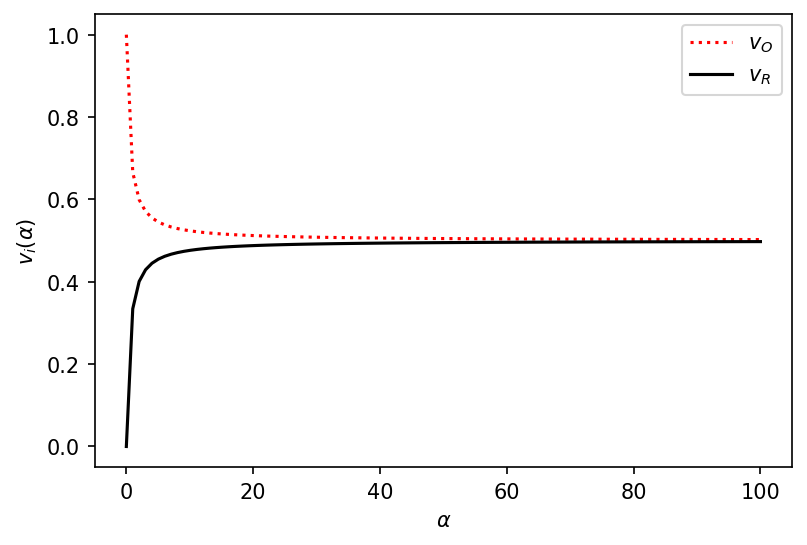
\includegraphics[scale=0.56]{figs/bergaining_game.png}
		\caption{Juego del ultimátum en equilibrio. Cuando $\alpha \rightarrow \infty$, las ganancias de los jugadores se aproximan a una partición 50-50.}
		\label{fig:fig9}
	\end{figure}
	
	\textbf{c} - Por último, debemos describir las cantidades en equilibrio. Con un $\alpha = 0$, el jugador \textit{O} retiene todo, pero como se ve en la figura \ref{fig:fig9}, su función decrece con $\alpha > 0$. Esta función no tiene solución, pero podemos encontrar la asíntota cuando $\alpha \rightarrow \infty$. 
	
	Para \textit{R}: \vspace{-1cm}
	
	\begin{align*}
		\lim_{\alpha \rightarrow \infty} \frac{\alpha}{1 + 2 \alpha} & = \frac{\alpha}{\alpha \Big( \frac{1}{\alpha} + 2 \Big)} \\
		                                                             & = \frac{1}{( 0 + 2)} = \frac{1}{2}                       
	\end{align*}
	
	Este juego tiene interpretaciones interesantes. Cualquier intento de reducir el parámetro $\alpha$ producirá una partición que beneficie al oferente. Si hubiese una forma, y el jugador \textit{O} la conociera, usarla mejoraría su posición. Por ejemplo, justificar la desigualdad.
	
\end{exbox}

\subsection{Representación normal de juegos en forma extensiva}

Existe una forma de representar un juego estratégico en su forma normal, aunque esto requiere perder información temporal del juego. Volvamos al ejemplo de NoC.

\begin{figure}[H]
	\centering
	\footnotesize{
		\begin{forest} for tree={s sep=30pt}
			[Fer,circle,draw,fill=gray!20,label={[red]below:$x_0$},edge={->},
				[Ale,circle,draw,fill=gray!20,edge label={node[midway,left]{N}},label={[red]below:$x_1$},edge={->},
					[{2, 1},l=15mm, edge label={node[midway,left]{$n$}}]
					[{0, 0},l=15mm, edge label={node[midway,right]{$c$}}]
				]
				[Ale,circle,draw,fill=gray!20,edge label={node[midway,right]{C}},label={[red]below:$x_2$},edge={->},
					[{1, 2},l=15mm, edge label={node[midway,left]{$n'$}}]
					[{0, 0},l=15mm, edge label={node[midway,right]{$c'$}}]
				]
			]
		\end{forest}}
	\caption{Juego NoC en forma extensiva.}
	\label{fig:fig11}
\end{figure}

El perfil de estrategias que tiene Fer es $S_{Fer} = \{N, C\}$, mientras que el perfil de estrategias (por cada nodo) para Ale es $S_{Ale} = \{nn', nc', cn', cc' \}$. Por ejemplo, la primera estrategia $nn'$ corresponde a la estrategia ``escoger $n$ si Fer escoge N, o $n'$ si fer escoge C'', y así por el estilo.

Este juego puede ser representado (de nuevo, con pérdida de información temporal) por la siguiente tabla:

\begin{table}[H]
	\centering
	\begin{game}{2}{4}[Fer][Ale]
		&  $nn'$ & $nc'$ & $cn'$ & $cc'$  \\
		N  & $2, 1$  & $2, 1$ & $0, 0$ & $0, 0$\\
		C  & $0, 0$  & $1, 2$ & $0, 0$ & $1, 2$
	\end{game}
	\caption{Juego secuencial de NoC representado en forma normal.}
	\label{tbl:tbl6}
\end{table}

Dado que las estrategias de Ale se formulan \textit{antes} de que conozca el movimiento, tiene realmente 4 opciones por estrategia de Fer. 

% {\color{red}\rule{6cm}{2pt} stop}

\begin{exbox}{Ejercicios }%para resolver en clase - tarea (en caso de no alcanzar el tiempo)}
	
	\textbf{Ejercicio 1}
	
	Encontrar el equilibrio de estrategias mixtas (es decir, el perfil de estrategias $\sigma^*$ para cada jugador) así como los pagos (es decir, la utilidad $u_i(\sigma_i^*,\sigma_{-i}^*)$) para los siguientes juegos:
	
	\textbf{Ejercicio 1.2}\\
	\rule[15pt]{2.5cm}{1pt}
	
	\begin{center}
		\begin{game}{2}{2}[J1][J2]
			& izquierda     & derecha \\
			arriba   & $7, 2$  & $11,1$\\
			abajo    & $8, 7$  & $8,8$
		\end{game}
		        
	\end{center}
	
	\textbf{Ejercicio 1.3.} Si multiplicas las ganancias por una constante $\alpha > 0$, ¿el equilibrio del juego cambia? ¿Por qué sí o por qué no?
	
	\textbf{Ejercicio 2}\\
	\rule[10pt]{2.5cm}{1pt}
	
	\begin{figure}[H]
		\centering
		\begin{istgame}
			\xtdistance{15mm}{30mm}
			\istroot[-135](0)[initial node]<0>{J1}
			\istb{A}[a]{(2,2)}[l] \istb{D}[r] \endist
			\istroot(1)(0-2)<135>{J2}
			\istb{L}[al] \istb{R}[ar] \endist
			\xtdistance{10mm}{15mm}
			\istroot(2)(1-1)%<135>{J1}
			\istb{\ell}[al]{(3,3)} \istb{r}[ar]{(2,2)} \endist
			\istroot(3)(1-2)%<45>{J1}
			\istb{\ell}[al]{(4,2)} \istb{r}[ar]{(1,1)} \endist
			% \xtSubgameBox(1){(2-1)(3-2)}
			\xtInfoset(2)(3){J1}
		\end{istgame}
		\caption{Juego dinámico con información completa.}
		\label{fig:fig12}
	\end{figure}
	
	Encontrar:
	\begin{myenum}
		\item Subjuegos. Especificar las razones por las que un subjuego lo es.
		\item EN perfecto en subjuegos. Una acción por conjunto de información.
		\item Distinguir entre los pagos resultantes en ENPS y los perfiles de estrategia.
	\end{myenum}
	
	Nota: un juego con información imperfecta \textit{no necesariamente} requiere resolverse con estrategias mixtas (puede usarse EIEED o el método de 3 pasos).
	
\end{exbox}

\subsection{Tópicos de organización industrial}

\subsubsection{Publicidad y competencia}

Las empresas anuncian sus productos para aumentar su demanda. También pueden señalar defectos en los productos de sus competidores. En el primer caso hablamos de \textit{publicidad positiva}, en el segundo de \textit{publicidad negativa}. Por ejemplo, la empresa A podría acentuar las desventajas de la empresa B diciendo que sus productos tienen muchos fallos, causando que la demanda de B decrezca y la de A aumente. En otras estrategias, la empresa A podría hacer publicidad para que \textit{todas} las empresas aumenten su producción. Por ejemplo, fue el caso de Levi's al promocionar el uso de jeans (pantalones de mezclilla) , aumentando la demanda para todos los productores de jeans, no solo para Levi's. 

Pongamos por caso un \textit{prejuego} de un duopolio de Cournot. La empresa 1 comienza una campaña de publicidad antes de que las empresas compitan por el mercado. Debe seleccionar un nivel de publicidad $a\geq 0$. La publicidad puede incrementar el precio que los consumidores están dispuestos a pagar por el resultado de las dos empresas. Si el precio es

\[ p(Q) = a - q_1 - q_2 \]

Cuando E1 selecciona un nivel de publicidad $a$, la segunda empresa lo observa. Luego de esto, ambas (simultáneamente) seleccionan su nivel de producción. Asumir que las empresas, en la etapa del prejuego (antes de la competencia) producen a costo $c(q) = 0$, pero la empresa 1 debe pagar $2a^3/81$. Dado que $a$ puede ser cualquier número positivo, este juego tiene infinito número de subjuegos. 

\begin{exbox}{Solución a prejuego de Cournot}
	
	\vspace{6cm}	
	
\end{exbox}

\subsubsection{Pánico bancario}

\begin{mybox}[colback=red!20]{Glosario}
	Un \textbf{pánico bancario }se refiere a la retirada masiva de inversiones o dinero de un banco por creer que este se volverá insolvente. 
\end{mybox}

Dos inversores han depositado cada uno de ellos una cantidad $D$ en un banco. El banco invierte estos depósitos en un proyecto a largo plazo. Si se ve obligado a liquidar su inversión antes de que el proyecto madure, puede recuperar $2r$, en donde $D > r > D/2$. Si el banco deja que la inversión madure, el proyecto rendirá $2R$, con $R > D$ (evidentemente, $2r < 2R$, así que $R > D > r > D/2$, por lo que, podríamos decir provisionalmente, conviene dejar que el proyecto madure.

Existen dos fechas en las que los inversores pueden sacar su dinero: la fecha 1 es anterior a la maduración de la inversión, la fecha 2 es posterior. Si ambos inversores sacan su dinero, ambos reciben $r$. Si solo un inversor saca dinero en la fecha 1, ese inversor recibe $D$, y el otro $2r - D$, y se acaba el juego. Si ninguno saca su dinero en la fecha 1, el proyecto puede madurar y pasamos a la fecha dos, post-maduración. 

Llegados a la fecha 2, si ambos inversores sacan su dinero, cada uno recibe $R$, si solo uno de ellos saca su dinero, ese jugador recibe $2R - D$ y el otro $D$. Si ninguno saca su dinero, cada uno recibe $R$. 

\textbf{Resolver:}

\begin{myenum}
	\item Representar el juego en forma extensiva.
	\item Encontrar el ENPS y las ganancias del juego.
\end{myenum}

\begin{exbox}{Solución de pánico bancario}
	
	\begin{figure}[H]
		\centering
		
\tikzset{every picture/.style={line width=0.75pt}} %set default line width to 0.75pt        

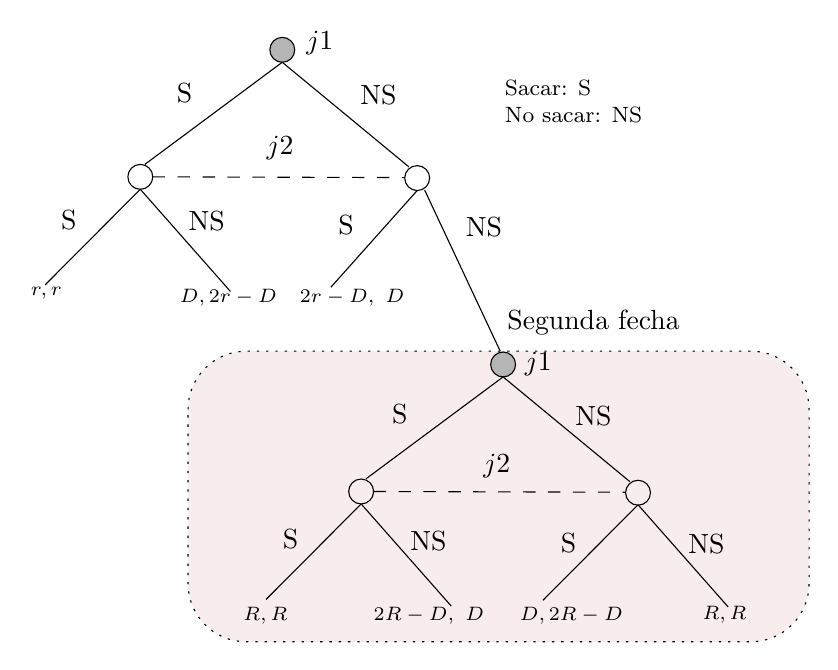
\begin{tikzpicture}[x=0.75pt,y=0.75pt,yscale=-1,xscale=1]
%uncomment if require: \path (0,300); %set diagram left start at 0, and has height of 300

%Rounded Rect [id:dp08510202990474469] 
\draw  [fill={rgb, 255:red, 247; green, 237; blue, 237 }  ,fill opacity=1 ][dash pattern={on 0.84pt off 2.51pt}] (220.6,183.2) .. controls (220.6,167.74) and (233.14,155.2) .. (248.6,155.2) -- (491.8,155.2) .. controls (507.26,155.2) and (519.8,167.74) .. (519.8,183.2) -- (519.8,267.2) .. controls (519.8,282.66) and (507.26,295.2) .. (491.8,295.2) -- (248.6,295.2) .. controls (233.14,295.2) and (220.6,282.66) .. (220.6,267.2) -- cycle ;
%Shape: Circle [id:dp16925021303630317] 
\draw  [fill={rgb, 255:red, 181; green, 181; blue, 181 }  ,fill opacity=1 ] (260,10) .. controls (260,6.69) and (262.69,4) .. (266,4) .. controls (269.31,4) and (272,6.69) .. (272,10) .. controls (272,13.31) and (269.31,16) .. (266,16) .. controls (262.69,16) and (260,13.31) .. (260,10) -- cycle ;
%Straight Lines [id:da18472788316592959] 
\draw    (266,16) -- (327,66.4) ;
%Straight Lines [id:da0058774636932865665] 
\draw    (199.8,65.2) -- (266,16) ;
%Shape: Circle [id:dp9080736926327866] 
\draw   (325,71.8) .. controls (325,68.49) and (327.69,65.8) .. (331,65.8) .. controls (334.31,65.8) and (337,68.49) .. (337,71.8) .. controls (337,75.11) and (334.31,77.8) .. (331,77.8) .. controls (327.69,77.8) and (325,75.11) .. (325,71.8) -- cycle ;
%Straight Lines [id:da6843039064749079] 
\draw    (289.4,124.4) -- (331,77.8) ;
%Shape: Circle [id:dp3828150651486175] 
\draw   (191.6,71.2) .. controls (191.6,67.89) and (194.29,65.2) .. (197.6,65.2) .. controls (200.91,65.2) and (203.6,67.89) .. (203.6,71.2) .. controls (203.6,74.51) and (200.91,77.2) .. (197.6,77.2) .. controls (194.29,77.2) and (191.6,74.51) .. (191.6,71.2) -- cycle ;
%Straight Lines [id:da4648615263287055] 
\draw    (197.6,77.2) -- (241,126.4) ;
%Straight Lines [id:da7149099866025843] 
\draw    (151.8,123.2) -- (197.6,77.2) ;
%Straight Lines [id:da8888487779527139] 
\draw  [dash pattern={on 4.5pt off 4.5pt}]  (203.6,71.2) -- (325,71.56) ;
%Straight Lines [id:da7323407395214239] 
\draw    (334.6,77.6) -- (371,155.2) ;
%Shape: Circle [id:dp5646143789453344] 
\draw  [fill={rgb, 255:red, 181; green, 181; blue, 181 }  ,fill opacity=1 ] (366.4,161.6) .. controls (366.4,158.29) and (369.09,155.6) .. (372.4,155.6) .. controls (375.71,155.6) and (378.4,158.29) .. (378.4,161.6) .. controls (378.4,164.91) and (375.71,167.6) .. (372.4,167.6) .. controls (369.09,167.6) and (366.4,164.91) .. (366.4,161.6) -- cycle ;
%Straight Lines [id:da9402607962677947] 
\draw    (372.4,167.6) -- (433.4,218) ;
%Straight Lines [id:da22954980795755042] 
\draw    (306.2,216.8) -- (372.4,167.6) ;
%Shape: Circle [id:dp6589878065353874] 
\draw   (431.4,223.4) .. controls (431.4,220.09) and (434.09,217.4) .. (437.4,217.4) .. controls (440.71,217.4) and (443.4,220.09) .. (443.4,223.4) .. controls (443.4,226.71) and (440.71,229.4) .. (437.4,229.4) .. controls (434.09,229.4) and (431.4,226.71) .. (431.4,223.4) -- cycle ;
%Shape: Circle [id:dp5747750920636694] 
\draw   (298,222.8) .. controls (298,219.49) and (300.69,216.8) .. (304,216.8) .. controls (307.31,216.8) and (310,219.49) .. (310,222.8) .. controls (310,226.11) and (307.31,228.8) .. (304,228.8) .. controls (300.69,228.8) and (298,226.11) .. (298,222.8) -- cycle ;
%Straight Lines [id:da08397429053648087] 
\draw    (304,228.8) -- (347.4,278) ;
%Straight Lines [id:da06721944707927507] 
\draw    (258.2,274.8) -- (304,228.8) ;
%Straight Lines [id:da6588726848749402] 
\draw  [dash pattern={on 4.5pt off 4.5pt}]  (310,222.8) -- (431.4,223.16) ;
%Straight Lines [id:da7199081913129757] 
\draw    (437.4,229.2) -- (480.8,278.4) ;
%Straight Lines [id:da26464014843372197] 
\draw    (391.6,275.2) -- (437.4,229.2) ;

% Text Node
\draw (143.6,123) node [anchor=north west][inner sep=0.75pt]  [font=\scriptsize]  {$r,r$};
% Text Node
\draw (215.4,124) node [anchor=north west][inner sep=0.75pt]  [font=\scriptsize]  {$D,2r-D$};
% Text Node
\draw (273.2,124.2) node [anchor=north west][inner sep=0.75pt]  [font=\scriptsize]  {$2r-D,\ D$};
% Text Node
\draw (246,277.4) node [anchor=north west][inner sep=0.75pt]  [font=\scriptsize]  {$R,R$};
% Text Node
\draw (379.2,277.4) node [anchor=north west][inner sep=0.75pt]  [font=\scriptsize]  {$D,2R-D$};
% Text Node
\draw (308.8,277.4) node [anchor=north west][inner sep=0.75pt]  [font=\scriptsize]  {$2R-D,\ D$};
% Text Node
\draw (467.2,277) node [anchor=north west][inner sep=0.75pt]  [font=\scriptsize]  {$R,R$};
% Text Node
\draw (373.2,134) node [anchor=north west][inner sep=0.75pt]   [align=left] {Segunda fecha};
% Text Node
\draw (372,23.6) node [anchor=north west][inner sep=0.75pt]  [font=\footnotesize] [align=left] {Sacar: S\\No sacar: NS};
% Text Node
\draw (214,25.2) node [anchor=north west][inner sep=0.75pt]   [align=left] {S};
% Text Node
\draw (302.4,26) node [anchor=north west][inner sep=0.75pt]   [align=left] {NS};
% Text Node
\draw (317.6,179.6) node [anchor=north west][inner sep=0.75pt]   [align=left] {S};
% Text Node
\draw (406,180.4) node [anchor=north west][inner sep=0.75pt]   [align=left] {NS};
% Text Node
\draw (158.2,86) node [anchor=north west][inner sep=0.75pt]   [align=left] {S};
% Text Node
\draw (219.6,86.8) node [anchor=north west][inner sep=0.75pt]   [align=left] {NS};
% Text Node
\draw (291.8,88.8) node [anchor=north west][inner sep=0.75pt]   [align=left] {S};
% Text Node
\draw (353.2,89.6) node [anchor=north west][inner sep=0.75pt]   [align=left] {NS};
% Text Node
\draw (265,240) node [anchor=north west][inner sep=0.75pt]   [align=left] {S};
% Text Node
\draw (326.4,240.8) node [anchor=north west][inner sep=0.75pt]   [align=left] {NS};
% Text Node
\draw (399,241.6) node [anchor=north west][inner sep=0.75pt]   [align=left] {S};
% Text Node
\draw (460.4,242.4) node [anchor=north west][inner sep=0.75pt]   [align=left] {NS};
% Text Node
\draw (276.4,-0.4) node [anchor=north west][inner sep=0.75pt]    {$j1$};
% Text Node
\draw (257.2,50.6) node [anchor=north west][inner sep=0.75pt]    {$j2$};
% Text Node
\draw (381.6,154.6) node [anchor=north west][inner sep=0.75pt]    {$j1$};
% Text Node
\draw (361.6,203.4) node [anchor=north west][inner sep=0.75pt]    {$j2$};


\end{tikzpicture}

		\label{fig:bank_run}
	\end{figure}
	
	1). Comenzamos con BI. Dado que la segunda fecha se trata de un subjuego que se puede jugar de forma simultánea, escribimos el juego como
	
	\begin{center}
		\begin{game}{2}{2}[j1][j2]
			& S     & NS \\
			S     & $R, R$  & $D,2R-D$\\
			NS    & $2R -D, D$  & $R, R$
		\end{game}
	\end{center}
	
	2). Sabemos que $R > D$, por lo tanto $R + R > D + R \Longrightarrow 2R - D > R$. Debido a esto, eliminamos la estrategia NS del jugador fila. Lo mismo sucede con el jugador columna.
	
	\begin{figure}[H]
		\centering
		

\tikzset{every picture/.style={line width=0.75pt}} %set default line width to 0.75pt        

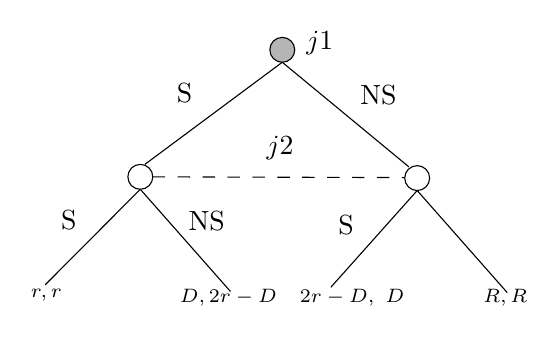
\begin{tikzpicture}[x=0.75pt,y=0.75pt,yscale=-1,xscale=1]
%uncomment if require: \path (0,300); %set diagram left start at 0, and has height of 300

%Shape: Circle [id:dp16925021303630317] 
\draw  [fill={rgb, 255:red, 181; green, 181; blue, 181 }  ,fill opacity=1 ] (260,10) .. controls (260,6.69) and (262.69,4) .. (266,4) .. controls (269.31,4) and (272,6.69) .. (272,10) .. controls (272,13.31) and (269.31,16) .. (266,16) .. controls (262.69,16) and (260,13.31) .. (260,10) -- cycle ;
%Straight Lines [id:da18472788316592959] 
\draw    (266,16) -- (327,66.4) ;
%Straight Lines [id:da0058774636932865665] 
\draw    (199.8,65.2) -- (266,16) ;
%Shape: Circle [id:dp9080736926327866] 
\draw   (325,71.8) .. controls (325,68.49) and (327.69,65.8) .. (331,65.8) .. controls (334.31,65.8) and (337,68.49) .. (337,71.8) .. controls (337,75.11) and (334.31,77.8) .. (331,77.8) .. controls (327.69,77.8) and (325,75.11) .. (325,71.8) -- cycle ;
%Straight Lines [id:da6843039064749079] 
\draw    (289.4,124.4) -- (331,77.8) ;
%Shape: Circle [id:dp3828150651486175] 
\draw   (191.6,71.2) .. controls (191.6,67.89) and (194.29,65.2) .. (197.6,65.2) .. controls (200.91,65.2) and (203.6,67.89) .. (203.6,71.2) .. controls (203.6,74.51) and (200.91,77.2) .. (197.6,77.2) .. controls (194.29,77.2) and (191.6,74.51) .. (191.6,71.2) -- cycle ;
%Straight Lines [id:da4648615263287055] 
\draw    (197.6,77.2) -- (241,126.4) ;
%Straight Lines [id:da7149099866025843] 
\draw    (151.8,123.2) -- (197.6,77.2) ;
%Straight Lines [id:da8888487779527139] 
\draw  [dash pattern={on 4.5pt off 4.5pt}]  (203.6,71.2) -- (325,71.56) ;
%Straight Lines [id:da4523012535261639] 
\draw    (331,77.8) -- (374.4,127) ;

% Text Node
\draw (143.6,124.2) node [anchor=north west][inner sep=0.75pt]  [font=\scriptsize]  {$r,r$};
% Text Node
\draw (215.4,124.2) node [anchor=north west][inner sep=0.75pt]  [font=\scriptsize]  {$D,2r-D$};
% Text Node
\draw (273.2,124.2) node [anchor=north west][inner sep=0.75pt]  [font=\scriptsize]  {$2r-D,\ D$};
% Text Node
\draw (214,25.2) node [anchor=north west][inner sep=0.75pt]   [align=left] {S};
% Text Node
\draw (302.4,26) node [anchor=north west][inner sep=0.75pt]   [align=left] {NS};
% Text Node
\draw (158.2,86) node [anchor=north west][inner sep=0.75pt]   [align=left] {S};
% Text Node
\draw (219.6,86.8) node [anchor=north west][inner sep=0.75pt]   [align=left] {NS};
% Text Node
\draw (291.8,88.8) node [anchor=north west][inner sep=0.75pt]   [align=left] {S};
% Text Node
\draw (276.4,-0.4) node [anchor=north west][inner sep=0.75pt]    {$j1$};
% Text Node
\draw (257.2,50.6) node [anchor=north west][inner sep=0.75pt]    {$j2$};
% Text Node
\draw (361.6,124.2) node [anchor=north west][inner sep=0.75pt]  [font=\scriptsize]  {$R,R$};


\end{tikzpicture}

		\label{fig:bank_run_sub}
	\end{figure}
	
	\begin{center}
		\begin{game}{2}{2}[j1][j2]
			& S     & NS \\
			S     & $r, r$  & $D,2r-D$\\
			NS    & $2r -D, D$  & $R, R$
		\end{game}
		        
	\end{center}
	    
	Sabemos que $r < D$, por lo tanto $r + r < D + r \Longrightarrow 2r - D < r$. Operando con la secuencia de 3 pasos, concluimos que este subjuego tiene dos equilibrios: $(S,S), (NS, NS)$ con ganancias de $(r, r)$ y $(R, R)$. El ENPS es entonces $\{(S, NS; S), (S, NS; S) \}$. 
	
	¿Cómo podemos interpretar esto? Una solución en este juego es eficiente y otra ineficiente, pero ambas suceden en equilibrio. Básicamente, no sabemos \textit{cuándo} podría ocurrir un pánico bancario, pero sabemos que podría ocurrir y que es una solución al juego. El problema es que conforme más gente retira su inversión, \textit{más probable} se vuelve la insolvencia del banco: la propia actitud ante el pánico causa la ruina misma que originalmente temían las personas, como una profecía autocumplida.
	
	La razón por la que ocurren los pánicos es porque la liquidez de los activos de los bancos como préstamos a privados es menor que la de sus obligaciones (depósitos a la vista, como la de las tarjetas o los retiros en cajero), y no podría hacer frente a la demanda de retiros debido a que su reserva es fraccionaria (solo mantiene una fracción de los depósitos de forma líquida). Una estrategia para evitarlo, analizada por el modelo de Diamond–Dybvig, es la suspensión de convertibilidad, en donde los bancos, bajo disposición contractual, en donde los bancos suspenden más retiros, lo que a su vez provoca más pánico. Debido a esto, se han propuesto seguros de depósitos por parte del Estado (en México existe el Instituto para la Protección del Ahorro Bancario, IPAB).  
	
\end{exbox}

\subsubsection{OS/2}

Cuando IBM decidió entrar al mercado de las PC en 1981, determinó hacer de su producto un estándar industrial. Para eso, subcontrató a otras compañías para la fabricación de componentes claves, incluyendo los microprocesadores y el sistema operativo (SO). Para el SO, recurrió a una \textit{pequeña} compañía llamada Microsoft, operada por Paul Allen y Bill Gates. 

Para satisfacer los requerimientos de IBM, Microsoft compró QDOS (Quick and Dirty Operating System) a la compañía Seattle Computer Products en 50k dólares, le hizo unas modificaciones y le dio el producto resultante a IBM como MS-DOS (Microsoft Disk Operating System). En lo que puede ser considerada una de las peores decisiones de negocios de la historia, IBM le permitió a Microsoft retener el copyright de MS-DOS, pensando en que el producto más rentable sería la PC en vez del SO. Sin embargo, las PC se convirtieron en un bien primario fungible, con muchos competidores entrando al mercado, mientras que Microsoft se volvió dominante en el mercado de software debido a MS-DOS, por la vía de los llamados \textit{efectos de red}, según el cual un producto tiene más valor para un consumidor entre más consumidores lo usen (e.g., un celular no tienen ningún valor si nadie lo usa; lo mismo una red social). 

Luego de reconocer su torpeza, IBM comenzó a desarrollar su propio SO, que fue liberado con el nombre de OS/2 en 1987, pero Microsoft ya había comenzado a liberar versiones de Windows, el principal competidor de OS/2. Sin embargo, la mayoría de las aplicaciones desarrolladas eran para Windows, por lo que muy pocos consumidores compraban OS/2. 

Para capturar el desafío de IBM, supongamos un juego donde IBM decide entre desarrollar OS/2 o no, y después de desarrollar OS/2, tres compañías más deciden si desarrollar aplicaciones para OS/2. Si las tres compañías desarrollan, IBM obtiene la mayor ganancia, de lo contrario, si ninguna desarrolla aplicaciones, IBM pierde. La Figura \ref{fig:fig13} muestra el desarrollo del juego.

\textbf{Resolver}


\begin{myenum}
	\item Encontrar el EN en subjuegos perfectos: perfil de estrategias y pagos.
	\item ¿Debería IBM desarrollar OS/2? Si sí, ¿qué podría suceder, de acuerdo a los perfiles de estrategias encontrados?
\end{myenum}

\begin{figure}[H]
	\centering
	\footnotesize{
		\begin{forest} decision tree,for tree={s sep=12pt, l sep=30pt}
			[IBM, plain content,
				[{0,0,0,0};NDevOS/2,plain content,elo={yshift=4pt},s=3.5cm]
				[C1;DevOS/2,plain content,elo={yshift=4pt}
					[C2;D,plain content,elo={yshift=4pt},alias=c2i
						[C3;{D,d},plain content,elo={yshift=4pt},alias=c30
							[{20, 3, 3, 3}; {D,d},elo={xshift=-3pt}]
							[{15, 1, 1, 0}; {ND,(1-d)}]
						]
						[C3;{ND,(1-d)},plain content,elo={yshift=4pt},alias=c31
							[{15, 1, 0, 1}; {D,d}]
							[{-2, -1, 0, 0}; {ND,(1-d)}]
						]
					]
					[C2;ND,plain content,elo={yshift=4pt},alias=c2d
						[C3;{D,d},plain content,elo={yshift=4pt},alias=c32
							[{15, 0, 1, 1}; {D,d}]
							[{-2, 0, -1, 0}; {ND,(1-d)}]
						]
						[C3;{NDev,(1-d)},plain content,elo={yshift=4pt},alias=c33
							[{-2, 0, 0, -1}; {D,d}]
							[{-3, 0, 0, 0}; {ND,(1-d)}]
						]
					]
				]
			]
			\draw[dashed,transform canvas={yshift=-6pt}] (c2i) to[right=45] (c2d);
			\draw[dashed,transform canvas={yshift=-6pt}] (c30) to[right=45] (c31) to[right=45] (c32) to[right=45] (c33);
		\end{forest}}
	\caption{C1 a C2 son compañías de desarrollo que deciden si desarrollar o no aplicaciones para OS/2. Como se trata de un juego con información imperfecta, el subjuego de C1 puede desarrollarse como un juego simultáneo. Si es un juego de estrategias mixtas, $d$ y $(1-d)$ denotan la probabilidad de desarrollar o no desarrollar.}
	\label{fig:fig13}
\end{figure}

\begin{exbox}{Solución a IBM: OS/2}
	
	Comenzamos con resolver el subjuego que comienza la decisión de C1, que debe decidir si desarrollar aplicaciones o no desarrollarlas. Su pago esperado por desarrollar es la suma ponderada de la probabilidad de desarrollo por la utilidad de desarrollo. En todos los casos, la utilidad de C1 es la segunda en orden. 
	
	Por la primera rama a la izquierda, si C1 desarrolla (D), obtiene 
	
	\[UE_{C1}(D) = \underbrace{d\times d \times 3}_{D,D,D} + \underbrace{(1-d)\times d \times 2}_{2(D,D,ND)} + \underbrace{(1-d)^2\times (- 1)}_{D, ND, ND} = 4d-1\]
	
	Dado que si no desarrolla no obtiene nada (pago de 0), igualando $UE_{C1}(D) = 0$ (estrategias mixtas), $d=1/4$. Por lo tanto, cada compalñía, en estrategias simétricas, decide desarrollar con probabilidad de $1/4$, y no desarrollar con $3/4$. (Recordar que resolvimos estrategias mixtas para $d$, inicialmente solo para C1, pero la $d$ encontrada también vale para C1).
	
	La ganancia esperada de IBM es entonces
	
	
	\begin{align*}
		UE_{IBM}(DevOS/2) = & \underbrace{d^3 \times 20}_{3~des.} + 3\times\underbrace{(d^2\times (1-d) \times 15 )}_{2~des.} + & 3\times \underbrace{(d \times (1-d)^2\times (-2))}_{2~no~des.} + \\
		& \underbrace{(1-d)^2 \times (-3)}_{3~no~des.}
	\end{align*}
	
	Sustituyendo nos da $UE_{IBM}(DevOS/2) = \frac{20}{64}$. Esto es ciertamente mejor que no desarrollar (0), sin embargo, IBM solo gana en el caso de que \textit{al menos} dos compañías desarrollen, un evento que sucede cuando desarrollan 3 ($d^3=(1/4)^3=1/64$) y cuando desarrollan 2 ($3d^2(1-d)=3(1/4)^2(3/4)=9/64$), es decir, $10/64$, mientras que la probabilidad de que IBM falle es de $54/64$.
	
\end{exbox}

\subsection{Regateo \textit{(bargaining)} y negociación}

\subsubsection{Conflicto laboral}

Una empresa planea hacer despidos masivos y recontratar a nuevo personal con menores salarios. Hacerlo implicaría enfrentarse a un conflicto laboral con el sindicato y negociar los términos de los despidos. El sindicato y la empresa pueden adoptar dos estilos de negociación: duro (Dr, dr) y blando (Bl, bl), aunque la empresa no sabe si el sindicato negociará de una forma u otra. Si alguno de los dos actúa de manera blanda y el otro se comporta negociando duramente, el primero no obtiene beneficio alguno (gana 0), mientras que el segundo se apropia de todos los beneficios ($b$). Sin embargo, los beneficios se reparten por mitad si ambos adoptan una actitud conciliadora, pero si los dos negocian agresivamente, ambos sufrirán un costo $c$, y en este caso cada uno obtendría $(b-c)/2$, con $c > b$. Por último, si la empresa decide no realizar los despidos, se queda con $b/3$ y y el sindicato con $2b/3$.

\textbf{Resolver}:

\begin{myenum}
	\item Representar como juego en forma extensiva.
	\item Encontrar para cual $c$ en términos de $b$ la empresa decidirá no realizar despidos.
\end{myenum}

\begin{exbox}{Solución a problema de conflicto laboral S vs E}
	
	\begin{minipage}{.5\textwidth}
		\begin{figure}[H]
			\centering
			\footnotesize{
				\begin{forest} decision tree,for tree={s sep=25pt}
					[E, plain content
						[{$\frac{1}{3}b$,$\frac{2}{3}b$};ND,plain content,elo={yshift=4pt}]
						[S;D,plain content,elo={yshift=4pt}
							[E;Bl,plain content,elo={yshift=4pt},alias=j2i
								[{\frac{b}{2},\frac{b}{2}};bl]
								[{b,0};dr]
							]
							[E;Dr,plain content,elo={yshift=4pt},alias=j2d
								[{0,b};bl]
								[{\frac{b-c}{2},\frac{b-c}{2}};dr]
							]
						]
					]
					\draw[dashed,transform canvas={yshift=-6pt}] (j2i) to[right=45] (j2d);
				\end{forest}}
			\caption{}
			% \label{fig:fig6}
		\end{figure}
	\end{minipage}%
	\begin{minipage}{.5\textwidth}
		\begin{center}
			\begin{game}{3}{3}[E][S]
				& Bl     & Dr & \( \sigma_E \) \\
				bl   & $\frac{b}{2}, \frac{b}{2}$  & $0,b$ & \cellcolor{blue!20} $q$ \\
				dr   & $b, 0$  & $\frac{b-c}{2},\frac{b-c}{2}$ & \cellcolor{blue!20} $1-q$ \\
				\( \sigma_S \) & \cellcolor{blue!20} $p$ & \cellcolor{blue!20} $1-p$ & 
			\end{game}
		\end{center}
		{\hspace{1.3cm} Subjuego comenzado en nodo de S}
	\end{minipage}
	
\end{exbox}

\begin{exbox}{Solución a problema de conflicto laboral S vs E (continuación)}
	
	El juego simultáneo se puede jugar con estrategias mixtas. Primero encontramos la el perfil de estrategias mixtas para E, $\sigma_E = \{ \sigma_E(bl), \sigma_E(dr) \}$
	
	\begin{align*}
		UE_{S}(Bl) & = p(b/2) + (1-p)0 = \frac{pb}{2}                        \\
		UE_{S}(Dr) & = pb + \frac{(1-p)(b-c)}{2}                             \\
		UE_{S}(BL) & = UE_{S}(Dr) = \frac{pb}{2} = pb + \frac{(1-p)(b-c)}{2} \\
		p          & = 1 - \frac{b}{c};\quad 1-p = \frac{b}{c}               
	\end{align*}
	
	Para S, el perfil de estrategias será el mismo: 
	
	\[q = 1 - \frac{b}{c};\quad 1 - q = \frac{b}{c} \]
	
	\begin{center}
		\begin{game}{3}{3}[E][S]
			&  $\sigma_E(bl)$             &  $\sigma_E(dr)$ & \( \sigma_E \) \\
			$\sigma_S(Bb)$ & $\Big(1 - \frac{b}{c} \Big)^2 \times \Big (\frac{b}{2}, \frac{b}{2}\Big )$  & $\Big[\Big(\frac{b}{c} - \Big (\frac{b}{c}\Big)^2 \Big] \times (0,b)$ & \cellcolor[gray]{0.9}  $1 - \frac{b}{c}$ \\
			$\sigma_S(dr)$ & $\Big[ \Big( \frac{b}{c} - \Big (\frac{b}{c}\Big)^2 \Big] \times (b, 0)$ & $ \Big[ \Big(\frac{b}{c}\Big)^2 \Big] \times \Big( \frac{b-c}{2},\frac{b-c}{2}\Big)$ & \cellcolor[gray]{0.9}  $\frac{b}{c}$ \\
			\( \sigma_S \) & \cellcolor[gray]{0.9} $1 - \frac{b}{c}$ & \cellcolor[gray]{0.9}  $\frac{b}{c}$ & 
		\end{game}
	\end{center}
	
	Suponer que $c=3, b=2$.
	
\end{exbox}

\subsection{Ventaja del primer movimiento}

\begin{exbox}{Stackelberg con dos empresas}
	Considerar a una empresa líder (L) y a una subordinada (F) en juego de competencia por cantidades de producción para producto homogéneo (mismo producto). 
	    
	La secuencia del juego es: 
	    
	\begin{itemize}
		\item Empresa L escoge una cantidad $q_1 \geq 0$.
		\item Empresa F observa $q_1$ y escoge una cantidad $q_2\geq 0$.
	\end{itemize}
	    
	Las empresas tienen una curva de demanda inversa:
	\[ P(Q) = a - Q\quad, \text{ con } Q = q_1 + q_2 \]
	    
	% En donde $Q$ es la cantidad agregada. La empresa líder tiene costo marginal $c_L > 0$, mientras que la empresa subordinada $c_F$, con el siguiente ordenamiento $1 > c_F \geq c_L$, que indica que la empresa líder tiene acceso a tec
	    
	El costo de la empresa $i$ por $q_i$ es $C_i(q_i)=cq_i$. Las funciones de ganancia conocidas:
	    
	\[u_i(q_i, qj)=q_i[a - (q_i + q_j) -c] \]
	    
	Encontrar el ENPS por inducción hacia atrás. 
	    
	\begin{myenum}
		\item Comenzamos con resolver para F para cualquier $q_1 \geq 0$ para encontrar la mejor respuesta $q_2(q_1^*)$. 
		\item Luego resolvemos para L.
	\end{myenum}
	    
	\[q_2^* = \argmax_{0\leq q2 \leq \infty} u_2(q_1, q_2) \]
	    
	CPO: $a - 2q_2 - q_1 - c = 0$
	    
	La mejor respuesta de F entonces es
	    
	\[ R_2(q_1) = (a - q_1 - c)/2\quad \text{ si } q_1 <a-c \]
	    
	Usamos $R$ para denotar que es una \textit{reacción} de F a L.
	    
	Ahora resolvemos para L. Notar que L también puede resolver el problema de F. O sea, L \textit{sabe} cuál podría ser la MR a su $q_1$. Debido a esto, el problema de L se resuelve si
	    
	\[q_1^* = \argmax_{0\leq q1 \leq \infty} u_2(q_1, R_2(q_1)) \]
	    
	O
	    
	\[q_1^* = \argmax_{0\leq q1 \leq \infty} q_1(a - q_1 - R_2(q_1) - c) \]
	
	Sustituyendo $R_2(q_1)$ en la función de L, la CPO es: 
	    
	\begin{align*}
		u_1(q_1, R_2(q_1)        & = q_1 \Big[a - q_1 -  \Big (\frac{a-q_1-c}{2}  \Big) - c \Big]                                  \\
		                         & =q_1 \Bigg (\frac{a}{2} - \frac{q_1}{2} -\frac{c}{2}\Bigg)                                      \\
		\frac{\partial u_1}{q_i} & = \frac{a}{2} - \frac{q_1}{2}-\frac{c}{2}\quad \text{ aplicando CPO }\frac{\partial u_1}{q_i}=0 \\
		q_1^*                    & = \frac{a-c}{2}                                                                                 
	\end{align*}
	    
	Si sustituimos $q_1^*$ en $R_2(q_1)$ nos queda que F escoge $q_2^* = \frac{a-c}{4}$.
	    
\end{exbox}

Para hacer el punto de la ventaja más claro, comparamos un juego de Cournot con su versión de Stackelberg. En ambos juegos los jugadores obtienen las mismas ganancias por decisión, sin embargo, las estrategias pueden ser distintas.

\begin{exbox}{Ventaja del primer movimiento: comparando Cournot con Stackelberg}

Un estudio de 1996 de Tellis y Golder \footnote{
	Tellis, G. J., \& Golder, P. N. (1996). First to market, first to fail? Real causes of enduring market leadership. \textit{MIT Sloan management review, 37(2), 65-75.}} encontró que, hasta ese año, solo cerca del \% 10 de las empresas innovadoras se convirtieron en líderes. Casos concretos son, por ejemplo, \textit{Chux}, que introdujo al mercado los pañales desechables (y terminó liderando \textit{P\&G}), o las grabadoras de cassette (introducida por Ampex, pero liderada por Matsushita y Sony). ¿Los primeros en mover entonces no tienen una ventaja? 
	
La tienen, pero la pueden perder. Haremos un ejemplo de un duopolio de Cournot con espacio de decisión discreto: uno como juego simultaneo y otro como un juego secuencial (aunque en este caso se sería un juego de Stackelberg, y el jugador que mueve primero es llamado líder \textit{Stackelberg}). El juego representado en la tabla \ref{tbl:tbl7} es uno donde escogen cantidades discretas el nivel de producción entre Alto, Mediano, Bajo y Nulo. Las ganancias se encuentran en cada celda para cada estrategia. Podemos verificar que la estrategia $(M, M)$ es un EN (usando EIEED).

\begin{table}[H]
	\centering
	\begin{game}{4}{4}[E1][E2]
		&  A    &     M    &     B   &  N   \\
		A  & $0, 0$  & $37.5, 25$ & $56.25, 28.125$ & $112.5, 0$ \\
		M  & $25, 37.5$  & $50, 50$ & $62.5, 46.875$ & $100, 0$ \\
		B  & $28.125, 56.25$ & $48.875, 62.5$ & $56.25, 56.25$ & $84.375, 0$ \\
		N  & $0, 112.5$ & $0, 100$ & $0, 84.375$ & $0,0$
	\end{game}
	\caption{Ganancias de E1 y E2.}
	\label{tbl:tbl7}
\end{table}

Con estos mismos pagos, en un juego extensivo, la empresa E1 (lídere Stackelber) tendría una ventaja si mueve primero.

\begin{figure}[H]
	\centering
	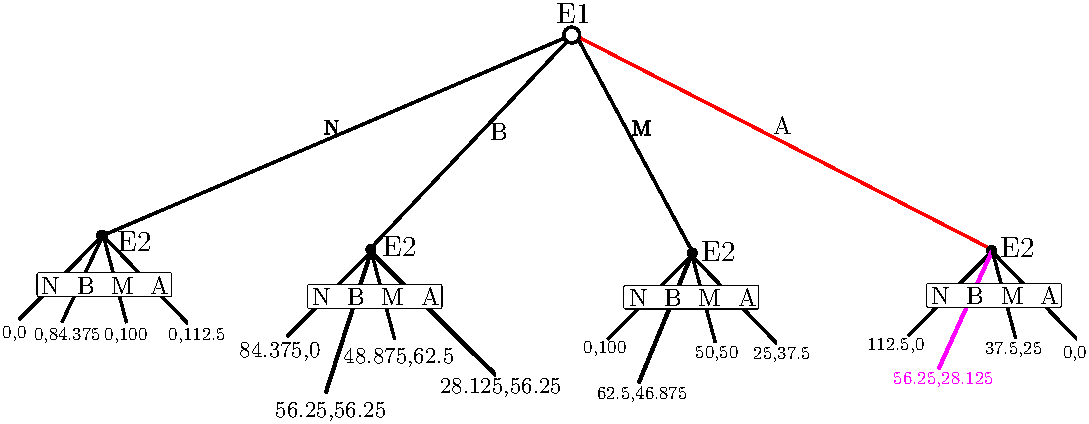
\includegraphics[scale=0.75]{figs/arbol_cournot.pdf}
	\caption{Juego en forma extensiva de un duopolio con cantidades discretas.}
	\label{fig:fig10}
\end{figure}

En este caso, la E2 podría tener más información que E1 en la segunda etapa de decisión, que podría explotar de alguna manera (e.g., reducir costos de producción del mismo producto, aumentar el nivel de publicidad, etc). Sin embargo, si no hace nada, esta información no supone una ventaja. 

\end{exbox}

Ahora desarrollamos un ejemplo similar al de IBM pero con una secuencia de juego distinta.

\begin{exbox}{Trabajo en clase: soluciones no únicas como escenarios posibles}
% Felix Seq-Move-Games, Ch4 p 134 1st ed

Normalmente, cuando encontramos soluciones no únicas, podemos adoptar estrategias mixtas y forzar solución única para encontrar las ganancias esperadas. Sin embargo, otra posibilidad es analizar los resultados del equilibrio como escenarios posibles: si ocurre un equilibrio vs si ocurre otro. Considerar el siguiente juego:

 Apple debe tomar la decisión de desarrollar un nuevo iPhone con nuevo software (radicalmente \textit{nuevo}) que permite nuevas y mejores aplicaciones, que no se han desarrollado aún. Si Apple no desarrolla el iPhone $\infty$, todas las compañías obtienen 0. Si Apple introduce el nuevo iPhone, la compañía 1, quien es líder de la industria de desarrollo, decide desarrollar aplicaciones compatibles. Luego de observar la decisión de la compañía líder, dos firmas subordinadas (2 y 3) deben decidir simultáneamente si desarrollar (D) o no (ND). 

Implementa el juego en su forma extensiva y encuentra el ENPS.

La forma extensiva del juego se encuentra en la Figura \ref{fig:apple_iphone}.

\begin{figure}[H]
	\centering
	\footnotesize{
		\begin{forest} decision tree,for tree={s sep=12pt, l sep=20pt}
			[Apple, plain content,
				[{0,0,0,0};\text{No iPhone 'nuevo'},plain content,elo={yshift=4pt},s=3.5cm,minimum width=4cm]
				[C1;\text{iPhone 'nuevo'},plain content,elo={yshift=4pt}
					[C2;D,plain content,elo={yshift=4pt},alias=c2i
						[C3;{D},plain content,elo={yshift=4pt},alias=c30
							[{10, 4, 4, 4}; {D},elo={xshift=-3pt}]
							[{6, 2, 2, 0}; {ND}]
						]
						[C3;{ND},plain content,elo={yshift=4pt},alias=c31
							[{6, 2, 0, 2}; {D}]
							[{-4, -2, 0, 0}; {ND}]
						]
					]
					[C2;ND,plain content,elo={yshift=4pt},alias=c2d
						[C3;{D},plain content,elo={yshift=4pt},alias=c32
							[{6, 0, 2, 2}; {D}]
							[{-4, 0, -2, 0}; {ND}]
						]
						[C3;{ND},plain content,elo={yshift=4pt},alias=c33
							[{-4, 0, 0, -2}; {D}]
							[{-6, 0, 0, 0}; {ND}]
						]
					]
				]
			]
			\draw[dashed,transform canvas={yshift=-6pt}] (c30) to[right=45] (c31);
			\draw[dashed,transform canvas={yshift=-6pt}] (c32) to[right=45] (c33);
		\end{forest}}
		\caption{}
	\label{fig:apple_iphone}
\end{figure}

La solución del juego se puede dar por inducción hacia atrás. Comenzando con los dos subjuegos que comienza C2. Para el caso en que y C1 Apple desarrollas, el juego tiene solución en estrategias puras, con ${(D,D), (4,4)}$. Para el caso en que C1 no desarrolla, tenemos dos EN: $(D,D)$ y $(ND,ND)$. 

Primero analizamos lo que sucede con  $(D,D)$ para el caso en que C1 no desarolla. 

\begin{figure}[H]
	\centering
	\footnotesize{
		\begin{forest} decision tree,for tree={s sep=12pt, l sep=20pt}
			[Apple, plain content,
				[{0,0,0,0};\text{No iPhone 'nuevo'},plain content,elo={yshift=4pt},s=3.5cm,minimum width=4cm]
				[C1;\text{iPhone 'nuevo'},plain content,elo={yshift=4pt}
					[{10, 4, 4, 4}; {D},elo={xshift=-3pt}]
					[{6, 0, 2, 2}; {ND}]
				]
			]
		\end{forest}%
		}
		\caption{Caso 1: C1 no desarrolla, pero C2 y C3 sí.}
	\label{fig:apple_ilose}
\end{figure}

Claramente, a C1 le conviene desarrollar. Si esto es cierto cuando ambas compañías C2 y C3 desarrollan, debe ser cierto cuando no desarrollan

\begin{figure}[H]
	\centering
	\footnotesize{
		\begin{forest} decision tree,for tree={s sep=12pt, l sep=20pt}
			[Apple, plain content,
				[{0,0,0,0};\text{No iPhone 'nuevo'},plain content,elo={yshift=4pt},s=3.5cm,minimum width=4cm]
				[C1;\text{iPhone 'nuevo'},plain content,elo={yshift=4pt}
					[{10, 4, 4, 4}; {D},elo={xshift=-3pt}]
					[{-6, 0, 0, 0}; {ND}]
				]
			]
		\end{forest}%
		}
		\caption{Caso 2: Ninguna desarrolla.}
	\label{fig:apple_ilose2}
\end{figure}

C1 sigue obteniendo más por desarrollar que por no desarrollar, independientemente de que las otras compañías desarrollen o no. Por inducción hacia atrás, el árbol para Apple es ahora

\begin{figure}[H]
	\centering
	\footnotesize{
		\begin{forest} decision tree,for tree={s sep=12pt, l sep=20pt}
			[Apple, plain content,
				[{0,0,0,0};\text{No iPhone 'nuevo'},plain content,elo={yshift=4pt},s=3.5cm,minimum width=4cm]
				[{10, 4, 4, 4};\text{iPhone 'nuevo'},plain content,elo={yshift=4pt}				]
			]
		\end{forest}%
		}
		\caption{Decisión de Apple}
	\label{fig:apple_ilose3}
\end{figure}

Ahora, la decisión de Apple es claramente desarrollar el iPhone `nuevo', dado que lo encuentra redituable. Si no forzamos el juego a estrategias mixtas, tenemos dos ENPS: ${(iPhone~Nuevo, D_{C1}, (D, D)_{C1/C2}, ((D, D)_{C1/C2})}$ y ${(iPhone~Nuevo, D_{C1}, (ND, ND)_{C1/C2}, ((ND, ND)_{C1/C2})}$. En ambos casos, las ganancias serán las mismas. Recordemos: un perfil de estrategias es un plan de acción, en donde una estrategia asigna una acción por nodo de decisión. La ruta del equilibrio no cambia porque incluso si las compañías 1 y 2 no desarrollan, desarrollar sigue siendo óptimo para C1.


\end{exbox}


\section{Juegos repetidos}

Un \textbf{juego repetido} es una situación en la que los jugadores tienen el mismo encuentro (conocido como \textit{juego de etapa (stage-game)}) una y otra vez. En un juego de ajedrez, por ejemplo, en cada periodo (cada movimiento) el juego es diferente. En un juego repetido no.

Sea $\delta \in [0, 1]$ el factor de descuento. Si se invierte una unidad (e.g., 1 peso) en el primer periodo se obtiene $1 + r$. Interpretamos $\delta$ como el una tasa a la que el valor del dinero disminuye \textit{debido a su potencial} de interés, entonces $\delta = 1/(1+r)$, en donde $r$ es el tipo de interés\footnote{
El monto por una inversión en un periodo $t$, en términos nominales, es inverso al monto en ese mismo periodo si el dinero no es invertido. En dos años, a una tasa de interés anual de $r$, una inversión $x_0$ valdrá $x_0(1+r)^2$. Por otro lado, si no invierto, una cantidad $v$ tendrá un valor presente en 2 años de $v=\frac{x_2}{(1+r)^2}$, precisamente porque $v$ es la cantidad que tendría que invertir \textit{ahora} para obtener $x_2$, porque $x_2=v(1+r)^2$.
}. 

En $T$ períodos sucesivos, el factor de descuento multiplica a a una cantidad en cada etapa $t$ que dure el juego. Si $u_i^{(t)}$ es la utilidad del jugador $i$ en la etapa $t$, el valor presente de una secuencia de ganancias será

\[ 
    u_i = u_i^{(1)} + \delta u_i^{(2)} + \delta^2 u_i^{(3)} + \dots + \delta^{t-1} u_i^{(t)} = \sum_{t=1}^{T}\delta^{t-1} u_i^{(t)}
\]

Si el juego durará $T$ periodos, podemos pensar en la cantidad de dinero como una cantidad \textit{esperada de dinero} después de $T$ encuentros. Si denotamos como $\delta$ la probabilidad de que el juego continúe y $1 - \delta$ como la probabilidad de que el juego termine, entonces la probabilidad de que el juego dure $t$ etapas está dada por la función de probabilidad de una distribución geométrica

\[ 
    p(t)=\delta^{t-1}(1-\delta)
\]

Es fácil probar esto. Sea $ \delta $ la probabilidad de $ X = 1 $ y $1-\delta$ la probabilidad de $ X = 0 $. Dado que cada etapa es esencialmente un ensayo de Bernoulli, si tenemos 4 etapas, tenemos 

\[
	\underset{\text{etapa 1}}{\delta} \times \underset{\text{etapa 2}}{\delta}\times \underset{\text{etapa } t - 1}{\delta}\times \underset{\text{etapa } t}{(1-\delta)}
\]

Y dado que cada ensayo es independiente, la probabilidad de que el juego dure 4 etapas es $ \delta^{t-1}\times(1-\delta) $

En una distribución geométrica, la cantidad de etapas esperadas que dura un juego es $\frac{1}{1-\delta}$. Para probar que una distribución geométrica tiene una esperanza $ \mathbb{E}[X] $ debemos encontrar el primer momento de la distribución geométrica usando su función generadora de momentos, $ M_X(k) = \mathbb{E}[e^{tX}]$. El primer momento es la media o esperanza.

\begin{align*}
	\mathbb{E}[X]&=\sum_{t=1}^{\infty}t(1-\delta)\delta^{t-1} \\
	&=(1-\delta)\sum_{t=1}^{\infty}t\delta^{t-1} \\
	&=(1-\delta)\left(-\frac{d}{d\delta}\sum_{t=1}^{\infty}\delta^t\right) \\
	&=(1-\delta)\left(-\frac{d}{d\delta}\frac{\delta}{(1-\delta)}\right) \\
	&=(1-\delta)\left(\frac{d}{d\delta}\left(1-\frac{1}{(1-\delta)}\right)\right)=(1-\delta)\left(\frac{1}{(1-\delta)^2}\right)=\frac{1}{1-\delta}
\end{align*}

Esta misma expresión se puede obtener de la siguiente forma: supongamos que un jugador puede obtener una unidad en cada periodo en un número infinito de periodos. La suma de sus ganancias descontadas es

\[ 
u = 1 + 1\delta + 1\delta^2 + \dots = 1 + \delta + \delta^2 + \dots
\]

Se puede simplificar si notamos que

\[ 
    \delta + \delta^2 + \dots = \delta(1 + \delta + \delta^2 + \dots) = \delta u
\]

Por lo tanto, $u=1+\delta u$, lo que significa 

\[u = \frac{1}{1-\delta} \]

el la cantidad esperada de etapas antes de que el juego termine. Esto a su vez implica que

\[ 
    u_i = u_i^{(1)} + \delta u_i^{(2)} + \delta^2 u_i^{(3)} + \dots + \delta^{t-1} u_i^{(t)} = \sum_{t=1}^{T}\delta^{t-1} u_i^{(t)} = \frac{u_i}{1-\delta}\quad \text{ para $T = \infty$}
\]

Que es la \textit{suma descontada de ganancia}, una utilidad esperada.

\begin{mybox}{Juego repetido}
    \begin{defi}
	    Definimos un juego repetido como un juego $J(T,\delta)$, con $T<\infty$, y en donde $J$ es un juego de escenario. El juego se repite $T$ veces y es finito. Si $T = \infty$ se dice que el juego se repite infinitas veces.
    \end{defi}
\end{mybox}

Las estrategias en un juego infinitamente repetido pueden crecer indeterminadamente, tomando en cuenta que una estrategia es una función que asigna una acción en cada conjunto de información de un jugador. Si cada jugador pasa por un infinito número de etapas, y en la etapa $t-1$ el la estrategia en ese conjunto es condicional a todas las etapas desde 1 hasta $t-1$. 

Sin embargo, no es necesario pasar por toda la ruta del juego. Dado que el mismo juego $J$ se repite indefinidamente, se pueden adoptar estrategias sencillas que también se repitan. Por ejemplo, elegir aquella que sea un EN en cada etapa del juego. Por ejemplo, en el dilema de los prisioneros, esta sería (D,D).

Usemos el ejemplo del dilema del prisionero

\begin{center}
    \begin{game}{2}{2}[1][2]
      &   C   &   D  \\
    C & (2,2) & (0,3)\\
    D & (3,0) & (1,1)
    \end{game}
\end{center}

Con este juego, capturaremos la idea de reputación. El intercambio que sucede entre, por ejemplo, un cliente y un comerciante es una situación estratégica. En un restaurante, por ejemplo, se puede vender un platillo con productos de buena o de mala calidad por el mismo precio. Si son de mala calidad, la ganancia sería mayor. Sin embargo, dado que entre el restaurante y los comensales se juegan juegos repetidos, el restaurante podría dañar su reputación, de forma que la siguiente ocasión el cliente o no vaya, o no esté dispuesto a gastar la misma cantidad, o peor: correr la voz. 

Consideremos una estrategia que llamaremos ``estrategia de activación''. En esta estrategia, dos acciones se ejecutan: cooperar y castigar. El perfil de castigo se asume que es el EN. Por otro lado, en la estrategia de activación los jugadores se comprometen a cooperar en cada periodo, pero si uno de ellos se desvía, entonces el otro juega castigo por siempre. Jugar D destruiría la reputación del jugador, y activaría el perfil de castigo (que es el EN del juego).

La estrategia de activación para el dilema del prisionero es jugar (C,C) siempre que sea lo que se ha jugado en el pasado, o cambiar a (D,D) en caso contrario. ¿Es un ENPS? Consideremos al jugador $i=1, 2$ en el periodo 1. El jugador $j$ se comporta de acuerdo a la estrategia de activación. En este caso, $i$ obtiene

$$u_i(s_i, s_j)=2 + 2\delta + 2\delta^2 + \dots = \frac{2}{1-\delta}$$

Si el jugador $i$ pudiera denunciar (D) en el primer periodo, le daría una ventaja inmediata de $3$ (porque se juega (D,C)), dado que $j$ juega C. Sin embargo, en el segundo periodo $j$ ya no juega más $C$, por lo que lo mejor que puede hacer $i$ es seguir jugando D hasta el final del juego. Por jugar D en el primer periodo, la suma descontada de ganancias de $i$ sería

$$u_i(s_i, s_j)=3 + \delta + \delta^2 + \dots = 3 + \delta(1 + \delta + \delta^2 + \dots) = 3 + \frac{\delta}{1-\delta}$$

Si

\[
\frac{2}{1-\delta} \geq 3 + \frac{\delta}{1-\delta}
\]

entonces $i$ obtiene más si juega C perpetuamente que jugando D en el primer periodo. Simplificando esta desigualdad, nos queda $\delta \geq 1/2$. Así, los jugadores no tienen un incentivo extra por hacer trampa (contra la estrategia con la que se comprometieron) en el primer periodo \textit{siempre que} $\delta \geq 1/2$ (de hecho, en ningún periodo). 

¿Cómo interpretamos $\delta$? En cierta forma, es un factor que permite medir qué tanto peso tiene el pasado/futuro para un agente. Dado que $\delta \in [0, 1)$, su punto medio se encuentra en 1/2. Debajo de ese valor, el presente tiene más peso; por arriba de ese valor, el futuro tiene más peso. En el primer caso, se dice que un agente es impaciente (o hasta impulsivo), en el segundo caso, se dice que es paciente (o autocontrolado). ¿Qué pasa si $\delta = 0$? En ese caso, el resultado es el del primer juego. El juego termina en $1/(1-0)$ etapas\footnote{Porque la cantidad promedio de juegos jugada sería de $1/(1-\delta)$}. Las ganancias son, si el jugador $j$ juega C, de

\[ 3 + \frac{\delta}{1-\delta} = 3 + \frac{\delta}{1-0} = 3 \]

De manera que al estrategia de activación no sería un equilibrio (el jugador $j$ no tendría incentivos para jugar esa estrategia, por lo que, tanto como el $i$ se desviaría, y el equilibrio sería realmente (D,D)). Esto muestra que, en juegos de reputación, las decisiones de un jugador en un periodo $t+1$ dependen de lo hecho por todos en $t$, y sus ganancias son una combinación de dos: la ganancia presente y la ganancia de \textit{continuación}: $u_i^{(t)} + \delta u_i^{(t+1)}$.

\subsection{Reputación: Henry Ford y el salario de \$5 al día}

En 1914 Ford ofreció la cantidad inaudita de \$5 dólares al día en sus fábricas. Esto sucedió en un momento en el que la industria de automóviles pagaba \$2.25/día. Se puede concluir que Ford fue generoso con sus trabajadores, pero esta estrategia podría haber aumentado su ganancia.

Si un empleado trabaja para Ford, puede decidir si trabajar duro u holgazanear. asumamos que el costo monetario de un trabajador es \$1 por trabajar duro y 0 por holgazanear. Si el trabajador recibe un salario $w$, una ganancia de un periodo es $w$ si holgazanea y $w-1$ si trabaja duro. El salario del trabajador es su valor \textit{presente} de pagos de único periodo, con un factor de descuento $\delta$. 

Las ganancias de Ford es el valor presente de ganancias por trabajador, en donde $\beta$ es su factor de descuento. Suponer que su compañía tiene ingresos de \$4 por día de un trabajador que holgazanea y \$7 de uno que trabaja duro. Por ejemplo, si Ford ofrece un salario de \$5 y el trabajador holgazanea (y es despedido), pero un nuevo trabajador trabaja duro, la ganancia de Ford sería

\[ 
	\underbrace{4-5}_{\text{holgazán}}+\underbrace{\beta(7-5)+\beta^2(7-5)+\dots}_{\text{diligente}}=-1 + \beta\Bigg (\frac{2}{1-\beta} \Bigg )
\]

Asumir que es un suministro ilimitado de trabajadores dispuestos a trabajar por \$5/día. Asumir también que ha´y un suministro ilimitado de trabajos ofrecidos por otras compañías, de tal forma que un trabajador que es despedido siempre puede encontrar un nuevo trabajo con una posición que paga \$3 y tolera la holgazanería. Ford decide qué salario pagar y si (o si no) despedir a un trabajador. Si despide a uno, inmediatamente contrata a otro (para el siguiente periodo, el holgazán despedido es sustituido). 

Ford ofrece el contrato a sus trabajadores: pagar \$5 y continuar el contrato siempre que sean diligentes. Si holgazanea, se te identifica como un holagazán y eres despedido. La estrategia del trabajador es trabajar duro si se le paga \textit{al menos} \$5. Cualquier cantidad menor provoca que holgazanee.

Notar que Ford es indiferente entre que sus trabajadores sean holgazanes o diligentes, dado que los trabajadores son perfectos sustitutos (cantidad ilimitadas de ambos, por lo que un trabajador puede ser perfectamente sustituido por otro sin agotar la reserva de los diligentes). Despedir a un holgazán y retener a un diligente es óptimo (no tiene incentivos extra para desviarse de esa estrategia). Ahora ¿es óptimo ofrecerles \$5? (podemos hacerlos la pregunta general de si es óptima una estrategia en donde se intercambie algún aspecto del bienestar del trabajador (incluyendo la reducción de horas de trabajo) por la diligencia y eficiencia del trabajo; por ejemplo, ¿cómo se seleccionó la jornada de 8/día?). Suponer que ofrece $w$, y luego actúa de acuerdo a su estrategia en el futuro (ofrece \$5), y sus trabajadores actuán según su estrategia (menos que \$5 holgazanean, etc), Ford gana de acuerdo a

\begin{align*}
	(7-w) + \beta\Bigg (\frac{2}{1-\beta} \Bigg )\quad & \text{ si } 5 \leq w     \\
	(4-w)+\beta\Bigg (\frac{2}{1-\beta} \Bigg )\quad   & \text{ si } 3 \leq w < 5 \\
	\beta\Bigg (\frac{2}{1-\beta} \Bigg )\quad         & \text{ si } w \leq 3     
\end{align*}

Si el salario es al menos 5, el trabajador es diligente, y Ford obtiene $7-w$ (actual) y, actuando de acuerdo a esta estrategia en el futuro, obtiene $\beta (2 / (1-\beta)$ en el juego de continuación. Si $w$ está entre 3 y 5, el trabajador holgazanea, así que la ganancia actual de Ford es $4-w$, con el mismo pago futuro. Si $w$ es menor que 3, ningún trabajador estará dispuesto a trabajar para Ford (ahora, ya que hay otras compañías que pagan 3 sin importar si son holgazanes), por lo que la ganancia de Ford es 0, y en el futuro $\beta (2 / (1-\beta)$ (asumiendo que cambia de estrategia en el segundo periodo). 

Claramente, pagar 5 es mejor que pagar 3, y pagar 3 es mejor que pagar menos de 3. Ford pagará 5 si

\[ 
    2 + \beta\frac{2}{1-\beta} \geq 1 + \beta\frac{2}{1-\beta} \Longrightarrow 2\geq 1
\]

La prima del salario por pagar 5 es mayor que por pagar 3, pero podría ser \textit{por lo menos igual}, así que Ford no tiene ningún incentivo para desviarse.

Considerar ahora a un trabajador diligente. Si ganancia por trabajar duro es $u=w - 1$. Prefiere ser diligente a holgazán si\footnote{
Recordar que la suma de utilidad descontada es $u\frac{1}{1-\delta}$.
}

\[ 
    \frac{5-1}{1-\delta} \geq 5 + \delta \frac{3}{1-\delta} \Longrightarrow \frac{1}{2}
\]

Siempre que su factor de descuento sea mayor que 1/2, será diligente. Esta estrategia pudo haber hecho que Ford indujera el trabajo diligente, o que obtuviera una alta proporción de trabajadores diligentes.

\subsection{Colusión de Cournot}

% \begin{exbox}
%     A continuación se analiza un juego en forma extensiva que ayuda a entender el surgimiento de la violencia en el proceso de desintegración de Yugoslavia. En concreto, el modelo de James Fearon intenta dar las claves del enfrentamiento que tuvo lugar entre serbios y croatas a raíz de la declaración de independencia de Croacia con respecto a la federación yugoslava. (Sánchez-Cuenca).
% \end{exbox}

\end{document}